\documentclass[a4paper,12pt]{article}

\usepackage[utf8]{inputenc}
\usepackage[english]{babel}
\usepackage{mathtools}     % it also loads amsmath
\usepackage{amssymb}       % it also loads amsfonts
\usepackage{bm}            % bold Greek letters
\usepackage{xfrac}         % slanted fraction
\usepackage{bookmark}      % links and bookmarks
\usepackage{lmodern}       % font
\usepackage{fix-cm}        % arbitrary font size
\usepackage{authblk}       % authors block
\usepackage{array}         % extending tabular environment
\usepackage{subcaption}    % sub-figures
\usepackage{float}         % placing figures
\usepackage{framed}        % framed environment with right alignment
\usepackage[toc]{appendix} % changing numbering to capital letters
\usepackage{cite}
\usepackage{ulem}
\usepackage{ifthen}
\usepackage[usenames,dvipsnames]{xcolor}

\newboolean{show_comments}
\setboolean{show_comments}{true}
\newcommand\Ignasi[1]{\ifthenelse{\boolean{show_comments}}{\textcolor{blue}{#1}}{}}
\newcommand\Miguel[1]{\ifthenelse{\boolean{show_comments}}{\textcolor{red}{#1}}{}}

\newboolean{show_corregit}
\setboolean{show_corregit}{false}
\newcommand\IgnasiCorregit[1]{\ifthenelse{\boolean{show_corregit}}{\textcolor{blue}{#1}}{}}

\newcommand{\pder}[2]{\frac{\partial#1}{\partial#2}}
\newcommand{\ppder}[2]{\frac{\partial^2#1}{\partial#2^2}}
\newcommand{\abs}[1]{\lvert#1\rvert}
\newcommand{\norm}[1]{\lVert#1\rVert}
\newcommand{\defeq}{\mathrel{\vcenter{\baselineskip0.5ex\lineskiplimit0pt\hbox{\scriptsize.}\hbox{\scriptsize.}}}=}
\newcommand{\keywords}[1]{\textit{Keywords -} #1}
\renewcommand\Affilfont{\itshape\small}

\makeatletter
\newcommand{\pushright}[1]{\ifmeasuring@#1\else\omit\hfill$\displaystyle#1$\fi\ignorespaces}
\newcommand{\pushleft}[1]{\ifmeasuring@#1\else\omit$\displaystyle#1$\hfill\fi\ignorespaces}
\makeatother

\newcolumntype{+}{>{\global\let\currentrowstyle\relax}}
\newcolumntype{^}{>{\currentrowstyle}}
\newcommand{\rowstyle}[1]{\gdef\currentrowstyle{#1}#1\ignorespaces}

\title{A FIC-FEM procedure for the shallow water equations over partially wet domains}

\author[1,2]{Miguel Masó}
\author[1,2]{Ignasi de-Pouplana}
\author[1,2]{Eugenio Oñate}
\affil[1]{Centre Int. de Mètodes Numèrics a l'Enginyeria (CIMNE), Barcelona, Spain}
\affil[2]{Universitat Politècnica de Catalunya (UPC), Barcelona, Spain}

\begin{document}

\maketitle

\begin{abstract}
\noindent
\Ignasi{FALTA COMPLETAR. PARLAR DE LA NOVETAT (LA FORMULACIO ESTABILITZADA) I ELS 4 EXEMPLES QUE S'HAN RESOLT}
\Miguel{AMPLIAT. ES PROU? VAIG UNA MICA PERDUT AMB LES COSES GENERALS}
The aim of this paper is to develop a stable finite element formulation for the shallow water equations using the finite increment calculus (FIC) procedure.
This research is focused on the stability properties and only uses linear triangles for the spatial discretization with equal order of interpolation for all the variables.
The extension to higher order of polynomial interpolation functions and different geometries is straightforward.
The present FIC-FEM procedure is also able to design artificial viscosity for an adequate shock capturing.
A fully implicit time integration has been used and special attention has been payed to the dry domain in order to solve the moving boundaries with a fixed mesh eulerian approach.
Three academic examples and the simulation of an experiment are included in order to test the capabilities of this procedure.
The first simple examples test an specific feature such as the stability, the shock capturing and the dry-wet interface.
The last example is a simulation of an experiment and the results are compared with the reference.
%In this paper we present a stable finite element formulation for the shallow water equations. The FIC procedure is able to develop a stabilized formulation as well to design an artificial viscosity for an adequate shock capturing. This method is applied to partially wet domains.
\vspace{1em}

\Ignasi{KEYWORDS: shallow water equations, finite element method, FIC stabilization, dry-wetting model}

\noindent
\keywords{shallow water equations, finite element method, continuous Galerkin, FIC stabilization, dry-wetting model}
\end{abstract}


\section{Introduction}

\Ignasi{HAURIES DE COMENÇAR PARLANT UNA MICA DE LA MOTIVACIO DE LA RESOLUCIO D'AQUEST TIPUS D'EQUACIONS: QUÈ PERMETEN RESOLDRE QUE SIGUI RELLEVANT PER A LA SOCIETAT?, QUINA ÉS L'AVENTATGE DE FER-HO AMB METODES NUMERICS?, HI HA ALTRES MÈTODES (ANALITICS, ESTADISTICS, ETC.)?}
\Miguel{HE AFEGIT ALGUN PARÀGRAF}

The shallow water equations are often used to study the hydrological dynamics of rivers and estuaries or coastal hydrodynamics.
Derived from the vertical integration of the three-dimensional Navier-Stokes equations, the shallow water equations define an averaged free surface flow in the horizontal plane.
Due to the complexity of the geometry and the source terms is not possible to find an analytical solution for the PDE, and appears the need to design strategies to find numerical solutions.
In those physical phenomena, flooding or moving shoreline may occur, which is numerically defined by the null water depth.

The shallow water equations have traditionally been modelled using finite volumes because of its advantages of stability and monotonicity. Given its geometric flexibility and its natural way to introduce high order schemes, finite elements have been applied too \cite{zien3,navon1979,navon1988}.
However, since the finite elements exhibit spurious oscillations, the discontinuous Galerkin technique has been introduced \cite{ambati2007,khan2014,lee2019}.
It has the advantages of the geometrical flexibility of the finite elements and the stability of the finite volumes, but the introduction of high order schemes is not straightforward.
In order to prevent numerical instabilities in finite elements, stabilization, monotonic schemes or different order of polynomial interpolation can be explored \cite{hood1974,zien3,ortiz2012}.
%More recently, the discontinuous Galerkin \Ignasi{technique} has been introduced \Ignasi{[CITATIONS] \sout{,}. It \sout{which}} has the advantages of the geometrical flexibility of the finite elements and the stability of the finite volumes, but the introduction of high order schemes is not straightforward.
This research is focused in classical stabilized finite elements with equal interpolation order for all the variables and we will explore the capabilities of the finite increment calculus (FIC) to develop stable formulations for the shallow water equations.

Several families of stabilization methods can be found in the literature, usually applied to the convection-diffusion equations or Navier-Stokes equations. The most relevant are SUPG \cite{brooks1982},
ASGS\cite{codina1998}, GLS \cite{huges1989} and FIC\cite{onate1996,onate1998}.
Due to the hyperbolic character of the shallow water equations, a particular stabilization method for compressible flow or the Euler equations need to be developed.
The FIC-based stabilization has been applied to convection-diffusion, incompressible flows, among other applications \cite{onate1998,onate2001}\IgnasiCorregit{T'HE MODIFICAT AQUESTA CITA PER A QUE APAREGUIN VARIES CITES AGRUPADES (AMB EL PAQUET CITE ES POT FER. E.G. [2-4])}.
In those cases, where the convective term has an important role, a first order FIC term is enough to provide stability to the system.
However, the shallow water equations are governed by the convective term and the wave equation in a mixed formulation \cite{codina2008} and, in consequence, the common derivation of the FIC-based stabilization is not enough to provide stability in all the range of applicability of the shallow water equations. 
A generalization of this method is proposed in order to provide a global stability for the shallow water equations.

Once global stability is achieved, local instabilities may appear near discontinuities, which are inherent to the supercritical flows.
A local shock capturing was initially proposed by Huges \cite{huges1986} and a review of shock capturing techniques can be found in Codina \cite{codina2011}.
Other possibilities of the FIC-based formulations are explored to provide a shock capturing stabilization  \cite{cotela2016}. \Ignasi{AQUESTA ULTIMA FRASE NO L'HE ENTES. VOLS DIR QUE HAS EXPLORAT TERMES D'ALTRES FORMULACIONS FIC PER A ESTABILITZAR EL SHOCK CAPTURING? PODRIES POSAR AIXO EN UN ALTRE PARAGRAF I PARLAR DE L'ESTAT DE L'ART EN AQUESTA QUESTIO EN CONCRET} \Miguel{AIXÍ ÉS, ALTRES TERMES DE FIC PODEN INTRODUIR SHOCK CAPTURING.}

Additionally, the dry domain requires an accurate modeling because the hyperbolic equations require positive water depth in all the domain.
Several authors have proposed different methods to solve the shallow water equations with moving shoreline. Leclerc proposed an eulerian method \cite{leclerc1990} and later, Heniche et al. modified that method allowing the free surface to plunge under the topography \cite{heniche2000}.
Other authors developed a rough-porous layer \cite{candy2017,barros2011} or a modified depth integration \cite{defina2000}. Those approaches introduce new physical parameters in the balance equations.
En eulerian approach based on the work of Leclerc and Heniche is presented. \Ignasi{FALTA COMPLETAR UNA MICA L'ESTAT DE L'ART D'AQUEST PUNT} \Miguel{ESTAT DE L'ART AMPLIAT. ENCARA ES PODRIA PARLAR DELS MÈTODES LAGRANGIANS}

\Ignasi{AL FINAL HAURIES DE POSAR 1 PARAGRAF EXPLICANT COM S'ORGANITZA EL PAPER: PRIMER PRESENTES LES EQUACIONS DE GOVERN, DESPRES L'ESTABILITZACIO, EXEMPLES, ETC.} \Miguel{FET}

This article is organized as follows. Firstly the governing equations are presented.
In section \ref{sec:stabilization} the FIC procedure is applied to add the stabilization terms and the shock capturing terms.
In section \ref{sec:fem} the spatial and temporal discretizations are described.
The dry domain model is presented in the same section because it mainly depends on the discretization.
Section \ref{sec:examples} presents some numerical examples and the conclusions are given in section \ref{sec:conclusions}.

\section{Governing equations and linearization}

Let us start presenting the shallow water equations. They are the result of integrating vertically the Navier-Stokes equations, assuming the vertical velocity and its acceleration negligible \cite{abbot1979,zien3}.
\Ignasi{HAURIES D'EXPLICAR SI ESCRIUS LES EQUACIONS AMB VARIABLES CONSERVATIVES I PER QUÈ HO FAS AIXI AMB CITES}
\Miguel{TINC DUBTES IS ARA ÉS PROU O CALEN MÉS CITES. ALTRES AUTORS NO ACOSTUMEN A DEDICAR GAIRE TEMPS A EXPLICAR LES EQUACIONS.}
The equations governing the mass and momentum conservation can be written in conservative form with water depth $h$ and specific discharge $\mathbf{q}=(h\mathbf{u})$ as follows,

\begin{equation} \label{general_sw}
\pder{\Phi}{t} + \pder{\mathbf{F}_i}{x_i} + \pder{\mathbf{G}_i}{x_i} + \mathbf{Q} = \mathbf{0} \quad \text{for} \enspace i=1,2
\end{equation}
with

\begin{subequations}\label{variables_and_fluxes}
\allowdisplaybreaks
\begin{align}
\Phi &= \left\{
    \begin{array}{c}
        h \\
        hu_1 \\
        hu_2
    \end{array}\right\} \\
\mathbf{F}_i &= \left\{
    \begin{array}{c}
        hu_i \\ [5pt]
        hu_1u_i + \delta_{1i}\frac{1}{2}g(h^2 - z^2) \\ [5pt]
        hu_2u_i + \delta_{2i}\frac{1}{2}g(h^2 - z^2)
    \end{array}\right\} \\
\mathbf{G}_i &= \left\{
    \begin{array}{c}
        0 \\ [5pt]
        -(h/\rho) \bar{\tau}_{1i} \\ [5pt]
        -(h/\rho) \bar{\tau}_{2i}
    \end{array}\right\} \\
\mathbf{Q} &= \left\{
    \begin{array}{c}
        r \\ [5pt]
        \displaystyle -g(h-z)\pder{z}{x_1} + \frac{h}{\rho}\pder{p_a}{x_1}
        - \frac{1}{\rho}\tau^s_{31} + \frac{1}{\rho}\tau^b_{31} \\ [10pt]
        \displaystyle -g(h-z)\pder{z}{x_2} + \frac{h}{\rho}\pder{p_a}{x_2}
        - \frac{1}{\rho}\tau^s_{32} + \frac{1}{\rho}\tau^b_{32}
    \end{array}\right\}
\end{align}
\end{subequations}
where $\Phi$ is the vector of conserved variables, $\mathbf{F}$ is the vector of convective fluxes, $\mathbf{G}$ is the vector of viscous fluxes and $\mathbf{Q}$ is the vector source terms. In figure \ref{diagram} there is a representation of the variables and the notation. The coordinates are denoted with the index notation $x_i$, being $i=1,3$, while the number of dimensions $n_d$ is equal to 2. $\delta_{ij}$ is the Kronecker delta. The topography is expressed with the variable $z$ and the free surface elevation is expressed in terms of the topography and the total depth, $\eta = z + h$. $\bar{\tau}_{ij}$ are the averaged horizontal stresses, and $\tau^b_{3i}$ and $\tau^s_{3i}$ denote the bottom and surface friction stresses. Finally, $r$ is the rain source term and $p_a$ is the atmospheric pressure.

\Ignasi{AQUI HAURIES DE DEFINIR TOTES LES VARIABLES QUE ESTAS INTRODUINT A LES EQUACIONS 1 I 2, I EL SIGNIFICAT DE CADA EQUACIO (BALANÇ DE MASSA, MOMENT O EL QUE SIGUI). TAMBÉ HAURIES D'INDICAR D'ALGUNA MANERA FACIL QUE i ÉS CADA COMPONENT DE LES DUES DIMENSIONS AMB QUE MODELES EL DOMINI (TOT I QUE ARA S'ENTEN, EL PRIMER COP QUE HO HE LLEGIT M'HA SEMBLAT CONFUS)}
\Miguel{FET}

\begin{figure}
    \centering
    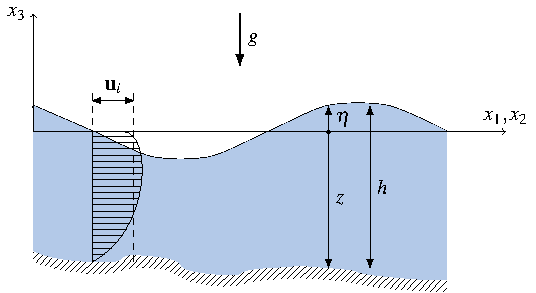
\includegraphics[width=.8\textwidth]{img/fig/diagram.pdf}
    \caption{Diagram and notation for the balance equations (\ref{general_sw}) and (\ref{variables_and_fluxes})}
    \label{diagram}
\end{figure}

The problem is closed with an initial boundary condition

\begin{equation}
\Phi = \Phi_0
\end{equation}
where $\Phi_0$ are the initial water height and specific discharge, verifying Equation (\ref{general_sw}), and the suitable\IgnasiCorregit{suitable} boundary conditions

\begin{align}
\Phi = \Phi_D \qquad &\text{in} \ \Gamma_D \\
\mathbf{F}_i\mathbf{n} = F_N \qquad &\text{in} \ \Gamma_N
\end{align}
where $\Gamma_D$ represents the part of the Dirichlet boundary conditions and $\Gamma_N$ represents the part of the Neumann boundary conditions. We will consider also absorbing boundary conditions ind $\Gamma_A$, such that $\Gamma_D \cap \Gamma_N \cap \Gamma_A = \delta\bm{\Omega}$.

The bottom friction $\tau^b_{3i}$\IgnasiCorregit{DEFINEIX (AQUÍ O ABANS) BOTTOM FRICTION COM } is modelled with the Manning formula \IgnasiCorregit{\sout{extended to} generalized for} generalized for two dimensions

\begin{equation}
\frac{\tau^b_{3i}}{\rho} = -gn^2\frac{\abs{\mathbf{u}}\mathbf{u}}{h^{\sfrac{4}{3}}}
\end{equation}

The averaged horizontal stresses are \IgnasiCorregit{calculated from the} calculated from the combination of the molecular stresses and the Reynolds stresses as follows

\begin{equation} \label{stresses}
\frac{\tau_{ij}}{\rho} = (\nu + \nu_t)\left(
    \pder{u_i}{x_j} + \pder{u_j}{x_i} -\frac{2}{3}\delta_{ij}\pder{u_k}{x_k} \right)
\end{equation}

The balance equation (\ref{general_sw}) is linearized in the following form

\begin{equation}
\pder{\Phi}{t} + \mathbf{A}_i\pder{\Phi}{x_i}
 - \pder{}{x_k}\left(\mathbf{K}_{ik}\pder{\Phi}{x_i}\right) + \mathbf{S}\Phi + \mathbf{F} = 0
\end{equation}
where the matrices $\mathbf{A}_i$ and $\mathbf{K}_{ik}$ are the linearization matrices of the convective fluxes and the diffusive fluxes. The convective matrices $\mathbf{A}_i$ \IgnasiCorregit{ET REFEREIXES A Ai?} are obtained after applying the chain rule to the vector of fluxes $\mathbf{F}_i$,
\begin{subequations}
\begin{align}
\pder{\mathbf{F}_i}{x_i} &= \pder{\mathbf{F}_i}{\Phi}\pder{\Phi}{x_i} \\
\mathbf{A}_i &= \pder{\mathbf{F}_i}{\Phi}
\end{align}
\begin{equation}
\mathbf{A}_1 = \left[\begin{matrix}
        2u_1 & 0   & -u_1^2 + c^2 \\
        u_2  & u_1 & -u_1 u_2 \\
        1    & 0   & 0
    \end{matrix} \right]
\quad , \quad
\mathbf{A}_2 = \left[\begin{matrix}
        u_1 & u_2  & -u_1 u_2 \\
        0   & 2u_2 & -u_2^2 + c^2 \\
        1   & 0    & 0
    \end{matrix} \right]
\end{equation}
\end{subequations}
and $c=\sqrt{gh}$ is the wave speed. The $\mathbf{A}_i$ matrix defines an hyperbolic ODE and its eigenvalues are $u+c$, $u$ and $u-c$, which requires positivity of the water column depth $h$.

And the bottom friction term is linearized using a reaction matrix $\mathbf{S}$
\begin{equation}
\mathbf{S} = \left[\begin{matrix}
    \frac{g\abs{\mathbf{u}}}{n^2h^{4/3}} & 0 & 0 \\
    0 & \frac{g\abs{\mathbf{u}}}{n^2h^{4/3}} & 0 \\
    0 & 0 & 0
\end{matrix}\right]
\end{equation}
In the following sections, the rain, atmospheric pressure gradient and the wind friction will be neglected. \IgnasiCorregit{SI AQUESTS TERMES JA HAN APAREGUT ABANS, ELS HAURIES D'HAVER DEFINIT, ENCARA QUE DESPRES NO APAREGUIN MÉS}

\section{Stabilization}\label{sec:stabilization}

We will consider the quasi-linear balance equations written in residual form as

\begin{equation} \label{residual}
r_j \defeq 
  \pder{\Phi}{t} + \mathbf{A}_i\pder{\Phi}{x_i}
  -\pder{}{x_k}\left(\mathbf{K}_{ik}\pder{\Phi}{x_i}\right) + \mathbf{S}\Phi + \mathbf{F} \qquad j\in\{1,n_d\}
\end{equation}

In the one dimensional case ($n_d=1$) \Ignasi{$n_d=1$ POTSER HAS DE DEFINIR AQUEST $n_d$ AL PRINCIPI AMB L'EQUACIO 1}\Miguel{FET}, the FIC-based stabilization has a unique definition and the stabilization parameter $l^e$ is usually the element length \cite{onate1998}

\begin{equation}
r - \frac{1}{2}l^e\pder{r}{x} = 0
\end{equation}

However, in two or three dimensional cases, or when the number of balance equations $n_b$ is different than $n_d$, the choice of the $l^e$ parameter is nontrivial.
Several approaches can be found in the literature. \cite{onate1998} took $l^e$ as a vector, but in later publications such as \cite{onate2001} a generalized formulation for different $n_d$ and $n_b$ was presented.
For the stabilization of the Navier-Stokes equations \cite{cotela2016} proposed different projections of the element size over the velocity and over the velocity gradient. To sum up, the different forms of the residual for the FIC stabilization can be written as

\begin{subequations}
\begin{align}
r_j - \frac{1}{2}l^e_i\pder{r_j}{x_i} &= 0
    \qquad i\in\{1,n_d\} \ ,\ j\in\{1,n_b\}\\[5pt]
r_j - \frac{1}{2}l^e_u\frac{u_i}{\norm{\mathbf{u}}}\pder{r_j}{x_i} &= 0
    \qquad i,j\in\{1,n_d\}\\[5pt]
r_j - \frac{1}{2}l^e_{g_i}\frac{\sfrac{\partial\mathbf{u}}{\partial x_i}}{\norm{\nabla u_i}}\pder{r_j}{x_i} &= 0
    \qquad i,j\in\{1,n_d\}
\end{align}
\end{subequations}

The FIC stabilization has been applied to problems with one balance equation (see \cite{onate1998} for the stabilization of the convection diffusion problem) or problems where the number of balance equations coincide with the number of space dimensions ($n_d = n_b$) (see \cite{onate1998} for the stabilization of the momentum and pressure equations of the Navier-Stokes equations). In this paper we propose a stabilization parameter which is oriented along the characteristics of the hyperbolic equations

\begin{equation} \label{fic_sw}
r_j - \frac{1}{2}l^e\frac{\mathbf{A}_i}{\lambda}\pder{r_j}{x_i}
    \qquad i\in\{1,n_d\} \ ,\ j\in\{1,n_b\}
\end{equation}
For consistency the linearization matrix $\mathbf{A}_i$ is normalized with the maximum eigenvalue $\lambda$. Note that this stabilization is analogue to the virtual multi-scale stabilization proposed in \cite{codina2008b}. The linearization matrix $\mathbf{A}_i$ provides a weighting procedure between the stabilization of the convective and the mixed wave equation terms. In practice the element size is multiplied by an algorithmic constant in order to control the amount of diffusion added by the stabilization and it will be studied in the examples of section \ref{sec:examples}.
\begin{equation} \label{fic_sw_beta}
r_j - \beta l^e\frac{\mathbf{A}_i}{\lambda}\pder{r_j}{x_i}
    \qquad i\in\{1,n_d\} \ ,\ j\in\{1,n_b\}
\end{equation}

The FIC formulation is the result of introducing the residual of the shallow water equations (\ref{residual}) into the expression in Eq (\ref{fic_sw_beta}). The variational expression of the equation is obtained by multiplying the equation by a test function $\omega_k$ and integrating over the domain $\Omega$ we obtain

\begin{equation} \label{variational_fic}
\int_\Omega \left(
    \omega_i r_j + \omega_k \beta l^e\frac{\mathbf{A}_i}{\lambda}\pder{r_j}{x_i}
\right) d\Omega = 0
\end{equation}
The second term of the expression (\ref{variational_fic}) is integrated by parts. Note that the element length $l^e$, the linearization matrix $\mathbf{A}_i$ and its eigenvalue $\lambda$ are defined constant inside the element, hence the boundary integral which appears after integrating by parts should be understood as the boundary of all the elements

\begin{equation} \label{variational_fic_parts}
\int_\Omega \omega_k r_j d\Omega
+ \int_\Omega \beta l^e\frac{\mathbf{A}_i}{\lambda}\pder{\omega_k}{x_i} r_j d\Omega
+ \sum_e \int_{\Gamma_e} \beta l^e\frac{\mathbf{A}_i}{\lambda}\omega_kn_kr_j d\Gamma = 0
\end{equation}
In this work we neglect the boundary integrals assuming that the residual $r_j$ is null at the boundary of the elements. At this point we introduce the balance equation (\ref{residual}) and integrate by parts the diffusive term

\begin{multline} \label{variational_balance_fic}
\int_\Omega \left(
    \omega_k \pder{\Phi}{t} + \omega_k \mathbf{A}_i\pder{\Phi}{x_i}
    + \pder{\omega_k}{x_j} \mathbf{K}_{jk} \pder{\Phi}{x_i} + \mathbf{S}\Phi + \mathbf{F}
\right) d\Omega\\ +
\int_\Omega \frac{\beta l^e}{\lambda} \left(
    \pder{\omega_k}{x_j} \mathbf{A}_j \pder{\Phi}{t}
    + \pder{\omega_k}{x_j} \mathbf{A}_j\mathbf{A}_i\pder{\Phi}{x_i}
    + \ppder{\omega_k}{x_j} \mathbf{A}_j\mathbf{K}_{jk} \pder{\Phi}{x_i} \right. \\
    \left.
    + \pder{\omega_k}{x_j} \mathbf{A}_j(\mathbf{S}\Phi + \mathbf{F})
\right) d\Omega
=0
\end{multline}
Equation \ref{variational_balance_fic} represents the stabilized formulation for the shallow water equations, similar to the expression obtained by SUPG. Note that the parameter $\beta l^e/\lambda$ is analogous to the characteristic time $\tau$ of the classical SUPG or GLS \cite{cotela2016}.

\subsection{Shock capturing}

In this section we explore other possibilities of the characteristic length definition in order to obtain a shock capturing stabilization. Here, the mass balance and the momentum balance are considered separately and the characteristic length is projected onto the gradient of the unknown

\begin{subequations} \label{eq:shock_capt}
\begin{align}
r_i^q + \frac{l^e}{2\norm{\nabla q_i}}\pder{q_i}{x_j}\pder{r_i^q}{x_j} &= 0 \label{eq:shock_capt_a}\\ 
r^h + \frac{l^e}{2\norm{\nabla h}} \pder{h}{x_j} \pder{r^h}{x_j} &=0 \label{eq:shock_capt_b}
\end{align}
\end{subequations}

Multiplying the momentum balance equation (\ref{eq:shock_capt_a}) by a proper test function $\omega_k$ , integrating over the domain in the same way as in equation \ref{variational_fic}, and then integrating by parts, one obtains its variational form:

\begin{align}    
\int_\Omega \omega_k r_i^q d\Omega
 - \int_\Omega \omega_k \frac{l^e}{2\norm{\nabla q_i}}\pder{q_i}{x_j}\pder{r_i^q}{x_j}
 d\Omega &= 0 \nonumber\\[5pt]
 \pushleft{\int_\Omega \omega_k r_i^q d\Omega} \nonumber\\
  + \int_\Omega \pder{}{x_j}\left(
      \omega_k \frac{l^e}{2\norm{\nabla q_i}}\pder{q_i}{x_j}
      \right)r_i^q d\Omega 
  - \int_\Omega \pder{}{x_j}\left(
      \omega_k \frac{l^e}{2\norm{\nabla q_i}}\pder{q_i}{x_j}r_i^q
      \right) d\Omega
    &= 0 \nonumber\\[10pt]
\pushleft{\int_\Omega \omega_k r_i^q d\Omega 
+ \int_\Omega \pder{\omega_k}{x_j}
    \frac{l^e r_i^q}{2\norm{\nabla q_i}}\pder{q_i}{x_j} d\Omega} \nonumber\\
+ \int_\Omega \omega_k \pder{}{x_j}\left(
     \frac{l^e}{2\norm{\nabla q_i}}\pder{q_i}{x_j}
    \right)r_i^q d\Omega 
- \int_\Omega \pder{}{x_j}\left(
    \omega_k \frac{l^e}{2\norm{\nabla q_i}}\pder{q_i}{x_j}r_i^q \right) d\Omega
    &= 0
\end{align}

After the integration by parts, the last two terms are dropped because they involve derivatives of the characteristic length\IgnasiCorregit{AQUI FALTA UNA PARAULA, O M'EQUIVOCO?} and can be transformed into a boundary integral. The same procedure is applied to the mass balance equation and we obtain the following expressions for both unknowns
\begin{subequations} \label{fic_shock_capturing}
\begin{align}
\int_\Omega \omega_k r_i^q d\Omega 
+ \int_\Omega \pder{\omega_k}{x_j}
\frac{l^e r_i^q}{2\norm{\nabla q_i}}\pder{q_i}{x_j} d\Omega &=0 \\
\int_\Omega \omega_k r^h d\Omega 
+ \int_\Omega \pder{\omega_k}{x_j}
    \frac{l^e r^h}{2\norm{\nabla h_i}}\pder{q_i}{x_j} d\Omega &=0
\end{align}
\end{subequations}

The above expressions (\ref{fic_shock_capturing}) are equivalent to a classical shock capturing method, which designs artificial diffusivity $k_{art}$ and artificial viscosity $\nu_{art}$

\begin{subequations} \label{k_art}
\begin{equation}
\nu_{art} = \frac{1}{2}\alpha l_e \frac{\abs{R(u_i)}}{\abs{\nabla u_i}}
\end{equation}
\begin{equation}
k_{art} = \frac{1}{2}\alpha l_e \frac{\abs{R(h)}}{\abs{\nabla h}}
\end{equation}
\end{subequations}
where $\alpha$ is an algorithmic constant.

Such approach can be refined by introducing the stabilization along the streamlines. This way, $k_{art}$ and $\nu_{art}$ need to be added only in the crosswind direction. The diffusive term is added with the following orthogonal tensor

\begin{equation}
\mathbf{D}_{art} = k_{art}
\left( \mathbf{I} - \frac{1}{\abs{\mathbf{u}}^2} \mathbf{u} \otimes \mathbf{u} \right)
\end{equation}
And the viscosity is introduced with a fourth order tensor in the crosswind direction using Voigt's notation:
\begin{subequations}
\begin{equation}
\mathbf{C}_{art} = \nu_{art} \mathbf{I}_4 \mathbf{O}
\end{equation}
\begin{equation}
\mathbf{O} = \left[\begin{matrix}
    1-\frac{q_1q_1}{\mathbf{q}\mathbf{q}} & -\frac{q_1q_2}{\mathbf{q}\mathbf{q}} & 0 \\
    -\frac{q_1q_2}{\mathbf{q}\mathbf{q}} & 1-\frac{q_2q_2}{\mathbf{q}\mathbf{q}} & 0 \\
    0 & 0 & 1-\frac{q_1q_2}{\mathbf{q}\mathbf{q}}
\end{matrix}\right]
\end{equation}
\end{subequations}
where $\mathbf{I}_4$ is the fourth order identity tensor for the stresses, which is derived from equation (\ref{stresses}) and will be defined in section \ref{sec:fem}\IgnasiCorregit{JO POTSER DEFINIRIA $\mathbf{I}_4$ AQUI PERO TAMPOC ES CRITIC AIXO}.

\section{Finite element formulation} \label{sec:fem} 

It is conventional to use higher order of interpolation for the momentum or velocity than for the water depth or free surface in order to develop stable finite elements formulations \cite{hood1974,heniche2000,bercovier1979}. In this research we restrict ourselves to use linear triangles for both $\mathbf{q}$ and $h$ unknowns, since the FIC-FEM procedure is stable. For that reason, all terms including spatial derivatives of order higher than two will be neglected. Bilinear quadrilaterals and higher order elements with the same number of degrees of freedom for all the variables will be also stables.

\subsection{Spatial discretization}

A finite element discretization $\Omega_h$ is introduced in the domain $\Omega$ and the problem variables can be interpolated with the basis functions of the finite elements space as

\begin{equation}
\phi_i = \sum_a^{N_\Omega} N_a(\mathbf{x})\phi_{ai}
\end{equation}
where $N_\Omega$ represents the total number of nodes in $\Omega_h$ and $\phi_i$ are the problem variables defined in (\ref{variables_and_fluxes}). Here we introduce the notation $\Phi_h$ for the vectors of nodal unknowns -momentum and water height- on all the finite element domain. The dot $\dot\Phi_h$ means temporal derivative. Following the Galerkin discretization, the shape functions $N_a$ are used to interpolate the test functions $\omega_k$ and the unknowns. The continuous equation (\ref{variational_balance_fic}) is combined with equation (\ref{fic_shock_capturing}) and can be expressed as the following algebraic system of equations
\begin{equation} \label{discrete_sw}
[\mathbf{M} + \mathbf{M}_K] \dot{\Phi}_h
+ [\mathbf{G} + \mathbf{G}_K + \mathbf{L} + \mathbf{L}_{SC} + \mathbf{R} + \mathbf{R}_K] \Phi_h
= \mathbf{F} + \mathbf{F}_K
\end{equation}
The matrices from equation (\ref{discrete_sw}) without subscript are related to the original problem (\ref{residual}), the matrices with subscript K correspond to the terms added by the FIC procedure to ensure stability, and those with the subscript SC are the terms added by the shock capturing. Using $a$, $b$ to denote the nodes, $i$, $j$ to denote the space dimension index and $k$, $l$ to denote the balance equation number, the matrices from equation (\ref{discrete_sw}) are defined as

\begin{align}
    \displaystyle \mathbf{M}^{ab} &= \int_{\Omega_e}N_a \mathbf{I} N_b d\Omega &
    \displaystyle \mathbf{G}^{ab} &= \int_{\Omega_e}
        N_a \mathbf{A}_i \pder{N_b}{x_i} d\Omega \nonumber\\[5pt]
    \displaystyle \mathbf{L}^{ab} &= \int_{\Omega_e}
        \mathbf{B}_a \left[\begin{matrix}
            \mathbf{C} & \mathbf{0} \\ \mathbf{0} & \mathbf{D}
        \end{matrix}\right] \mathbf{B}_b^T d\Omega &
    \displaystyle \mathbf{R}^{ab} &= \int_{\Omega_e} N_a \mathbf{S} N_b d\Omega \\[5pt]
    \displaystyle \mathbf{F}^{ab} &= \int_{\Omega_e} N_a gh\mathbf{z}_b d\Omega +
        \int_{\Gamma_e} N_a \mathbf{t}_b d\Gamma \nonumber
\end{align}
where the diffusive matrix $\mathbf{L}^{ab}$ is defined using the derivatives matrix $\mathbf{B}_a$ and the isotropic tensors $\mathbf{C}$ and $\mathbf{D}$

\begin{subequations}
\begin{equation}
\mathbf{B}_a = \left[\begin{matrix}
    \pder{N_a}{x_1} & 0 & \pder{N_a}{x_2} & 0 & 0 \\
    0 & \pder{N_a}{x_2} & \pder{N_a}{x_1} & 0 & 0 \\
    0 & 0 & 0 & \pder{N_a}{x_1} & \pder{N_a}{x_2}
\end{matrix}\right]
\end{equation}
\begin{equation}
\mathbf{C} = \nu \mathbf{I}_4 \ , \quad
\mathbf{D} = k \mathbf{I}_2 \ , \quad
\mathbf{I}_4 = \frac{1}{3} \left[\begin{matrix}
        2 & -1 & 0 \\
        -1 & 2 & 0 \\
        0 & 0 & 3
    \end{matrix}\right] \ , \quad
\mathbf{I}_2 = \left[\begin{matrix}
        1 & 0 \\
        0 & 1
    \end{matrix}\right]
\end{equation}
\end{subequations}

The stabilization and shock capturing terms from equation (\ref{discrete_sw}) result in analogous matrices with higher derivatives order, the boundary integral is neglected

\begin{align}
\displaystyle\mathbf{M}_K^{ab} &= \int_{\Omega_e} \frac{\beta l^e}{2} \pder{N_a}{x_i}\mathbf{A}_i N_b d\Omega &
\displaystyle\mathbf{G}_K^{ab} &= \int_{\Omega_e} \frac{\beta l^e}{2} \pder{N_a}{x_i}\mathbf{A}_i\mathbf{A}_j \pder{N_b}{x_j} d\Omega \nonumber\\
\displaystyle\mathbf{L}_{SC}^{ab} &= \int_{\Omega_e} \frac{\beta l^e}{2} \mathbf{B}_a \left[\begin{matrix}
        \mathbf{C}_\text{art} & \mathbf{0} \\ \mathbf{0} & \mathbf{D}_\text{art}
    \end{matrix}\right] \mathbf{B}_b^T d\Omega &
\displaystyle\mathbf{R}_K^{ab} &= \int_{\Omega_e} \frac{\beta l^e}{2} \pder{N_a}{x_i}\mathbf{A}_i \mathbf{S} N_b d\Omega \\
\displaystyle\mathbf{F}_K^{ab} &= \int_{\Omega_e} \frac{\beta l^e}{2} \pder{N_a}{x_i}\mathbf{A}_i gh\mathbf{x}_b d\Omega
\nonumber
\end{align}


\subsection{Temporal integration}

The resulting expression from the spatial discretization (\ref{discrete_sw}) can be written in the following compact form \IgnasiCorregit{JO NO UTILITZARIA EL MATEIX SIMBOL D'ABANS M, K, F AQUI. PODRIES POSAR UNS ALTRES SIMBOLS, e.g. $\tilde{\mathbf{M}}$,$\tilde{\mathbf{K}}$,$\tilde{\mathbf{F}}$}
\begin{equation} \label{discrete_compact}
\tilde{\mathbf{M}}\dot{\Phi}_h + \tilde{\mathbf{K}}\Phi_h = \tilde{\mathbf{F}}
\end{equation}
where the tilde symbol ($\,\tilde{}\,$) denotes the assembly of the system matrices for all the elements.
We have integrated this equation introducing a time discretization $t^n$ and using the well known BDF2 implicit scheme \cite{curtiss1952,brayton1972}. The system in a discrete time domain yields
\begin{equation}
\begin{split} \label{discrete_bdf2}
\tilde{\mathbf{M}}\dot{\Phi}_h^{n+1} + \tilde{\mathbf{K}}^{n+1}\Phi_h^{n+1} = \tilde{\mathbf{F}}^{n+1} \\
\dot{\Phi}_h^{n+1} = \beta_0 \Phi_h^{n+1} + \beta_1 \Phi_h^n + \beta_2 \Phi_h^{n-1}
\end{split}
\end{equation}
We will consider a variable time step to compute the BDF coefficients using the notation $t^{n+1} = t^n + \Delta t^n$:
\begin{equation}
\begin{split}
\beta_0 &= \tau (\rho^2 + 2\rho) \\
\beta_1 &= -\tau (\rho^2 + 2\rho + 1) \\
\beta_2 &= \tau
\end{split}
\end{equation}
with
\begin{equation}
\begin{split}
\tau &= \frac{1}{\Delta t^n(\rho^2 + \rho)} \\
\rho &= \frac{\Delta t^{n-1}}{\Delta t^n}
\end{split}
\end{equation}

The solution of this implicit system requires an iterative procedure which is defined in an incremental way as
$\Phi_h^{n+1,i+1} = \Phi_h^{n+1,i} + \delta\Phi_h^i$
where the superscript $i$ denotes the non linear iteration.\IgnasiCorregit{POTSER QUEDARIA MES CLAR SI POSES L'INDEX D'ITERACIO i A L'ESQUERRA DEL SIMBOL $^{i+1}\Phi_h^{n+1}$, TOT I QUE AIXO NO ES IMPORTANT} This notation allows us to rewrite the system of equations (\ref{discrete_bdf2}) defining a left hand side matrix multiplied by the increment $\delta\Phi_h^i$ and a right hand side vector which depends on the previous non linear iteration:
\IgnasiCorregit{FALTA EL SUPERINDEX i A LA K DEL LHS, CERT?}\Ignasi{AQUESTA ESTRATEGIA IMPLICITA ITERATIVA ES EL NEWTON-RAPHSON? O HI HA ALGUNA DIFERENCIA EN CONCRET?} \Miguel{ÉS NEWTON-RAPHSON}
\begin{equation}
[\beta_0\tilde{\mathbf{M}} + \tilde{\mathbf{K}}^{n+1,i}] \delta\Phi_h^i
= \tilde{\mathbf{F}}^{n+1,i} - \tilde{\mathbf{K}}^{n+1,i}\Phi_h^{n+1,i} - \tilde{\mathbf{M}}\dot{\Phi}_h^{n+1,i}
\end{equation}
The first non linear iteration $\Phi_h^{n+1,0}$ is initialized using a prediction given from the BDF formula at the last time step:
\begin{equation}
\Phi_h^{n+1,0} = \Phi_h^n + \Delta t^n \dot{\Phi}_h^{n}
\end{equation}


\subsection{Dry domain model}

When small or quasi zero water depths are involved in simulations, some instabilities may arise. In addition, the solution of the previous time integration scheme requires the inverse of a matrix which is singular in the dry regions. In this section we review the challenges associated to such problem, and the way we have circumvented them.

\paragraph{Recovery of the velocity field}
The first issue is the computation of the velocity field, since it involves the division of the discharge by the water height and this operation is ill-conditioned in the dry regions. In this research, the velocity field is computed in a two step procedure, first of all, the velocity is computed at each element following the next expression, initially proposed by Kurganov \cite{kurganov2007}:

\begin{equation} \label{h_inv_kurganov}
h^{-1}_k = \frac{\sqrt{2}\max(h,0)}{\sqrt{h^4 + \max(h^4, \varepsilon^4)}}
\end{equation}
where $\varepsilon$ is a threshold which depends on the elements size, usually $\varepsilon = 0.1 l_e$ is chosen. The second step in the velocity computation is a diffusive projection on the nodes: \IgnasiCorregit{QUE SON $\mathbf{M}_L$ I $\mathbf{M}_c$ ?}

\begin{equation}
\mathbf{M}_L \mathbf{u} = h^{-1}_k \mathbf{M} (h\mathbf{u})
\end{equation}
where $\mathbf{M}$ is the consistent mass matrix and $\mathbf{M}_L$ is the lumped mass matrix. This projection will introduce some artificial diffusion in the velocity field near the dry-wet interface reducing the possible maxima extrema.
Additionally, the expression(\ref{h_inv_kurganov}) tends to $0$ when the water height becomes small, while the analytical expression of the height inverse is recovered when $h>\varepsilon$.\IgnasiCorregit{QUE VOLS DIR AMB "while the original expression is recovered when $h>\varepsilon$" ? JO HO EXPLICARIA MES CLAR}


\paragraph{Partially wet elements}
At the elements where the shoreline is located, the interpolated water depth will not represent the real water surface.
Therefore those elements need an special consideration in order to prevent unrealistic oscillations. Excluding those elements from the computations is equivalent to introduce an artificial barrier, and the inclusion of those elements will incur in a consideration of an extra volume of water.
We chose to include all the elements in the computation and to modify the balance equations in order to satisfy equilibrium at rest (see figure \ref{partially_dry}). This is achieved by introducing a modified topography and imposing equilibrium:
\begin{equation}
    \pder{\eta'}{x_i} = \pder{z'}{x_i} + \pder{h}{x_i} = \mathbf{0}
\end{equation}

\begin{figure}
    \centering
    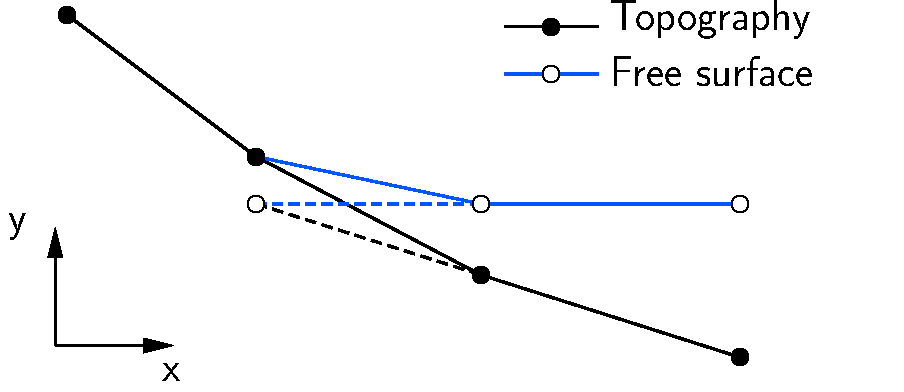
\includegraphics[width=.5\textwidth]{img/fig/partially_dry.pdf}
    \caption{Dry, wet and partially wet elements in the one dimensional case. The dashed line shows the modified topography  and the corresponding free surface.}
    \label{partially_dry}
\end{figure}

\paragraph{Avoiding the singularity of the system matrix}
Since all the elements are included in the computational domain, the last issue to overcome with small water depths is the singularity of the system matrix. The mass balance is satisfied in the dry state, but the momentum equation will become unstable. The easiest (although not the most accurate) way to develop a stable scheme is to add a diagonal of non zero terms to the momentum equation:

\begin{equation}
\mathbf{G} \defeq \mathbf{G} + \xi\,\text{diag}(1, 1, 0)
\end{equation}

The selection of the areas where there is a dry domain is controlled with a wet fraction function. The expression (\ref{h_inv_kurganov}) allows us to define a wet fraction $\omega$ as
\begin{equation}
\omega = hh^{-1}_k
\end{equation}
and so $\xi$ is defined as \IgnasiCorregit{CREC QUE EL SIMBOL $\alpha$ JA L'HAVIES UTILITZAT ABANS}
\begin{equation}
\xi = k(1-\omega)
\end{equation}
In our numerical experiments we have chosen $k=10^3$.
%See the figure \Ignasi{\sout{(}}\ref{inverse_heihgt}\Ignasi{\sout{)}}. \Ignasi{NO ACABO D'ENTENDRE QUÈ MOSTRES A LA FIGURA \ref{inverse_heihgt}}

\begin{figure}
    \centering
    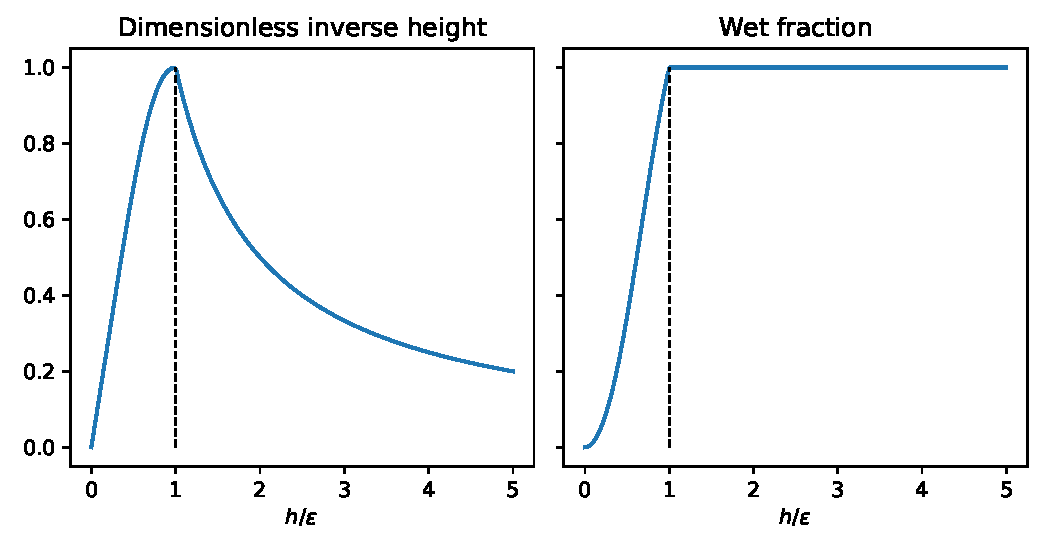
\includegraphics[width=\textwidth]{img/fig/inverse_height.pdf}
    \caption{Dimensionless functions to compute the  inverse height and the wet fraction.}
    \label{inverse_heihgt}
\end{figure}

%TODO: Ignasi - seguir per aqui

\section{Examples} \label{sec:examples}

This formulation has been implemented in KratosMultiphysics \cite{dadvand2010, dadvand2013}, an open source framework of numerical methods written in C++. Even thought Kratos implements triangles and quadrilaterals with several orders of interpolation \cite{kratos2020}, we have restricted ourselves to linear triangles in order to test the possibilities of the stabilization method. Each example is oriented to test a single aspect of the procedure explained in this research.



\subsection{Wave in a channel with a backward step}

The aim of the first example is to show that the Galerkin formulation applied to the shallow water equations is unstable and how the present stabilization method can overcome this issue and a calibration of the stabilization parameter is performed.
We study the propagation of a wave in a channel with a backward step. The wave is reflected at the end and faces the step in the opposite direction. 

\begin{figure}
    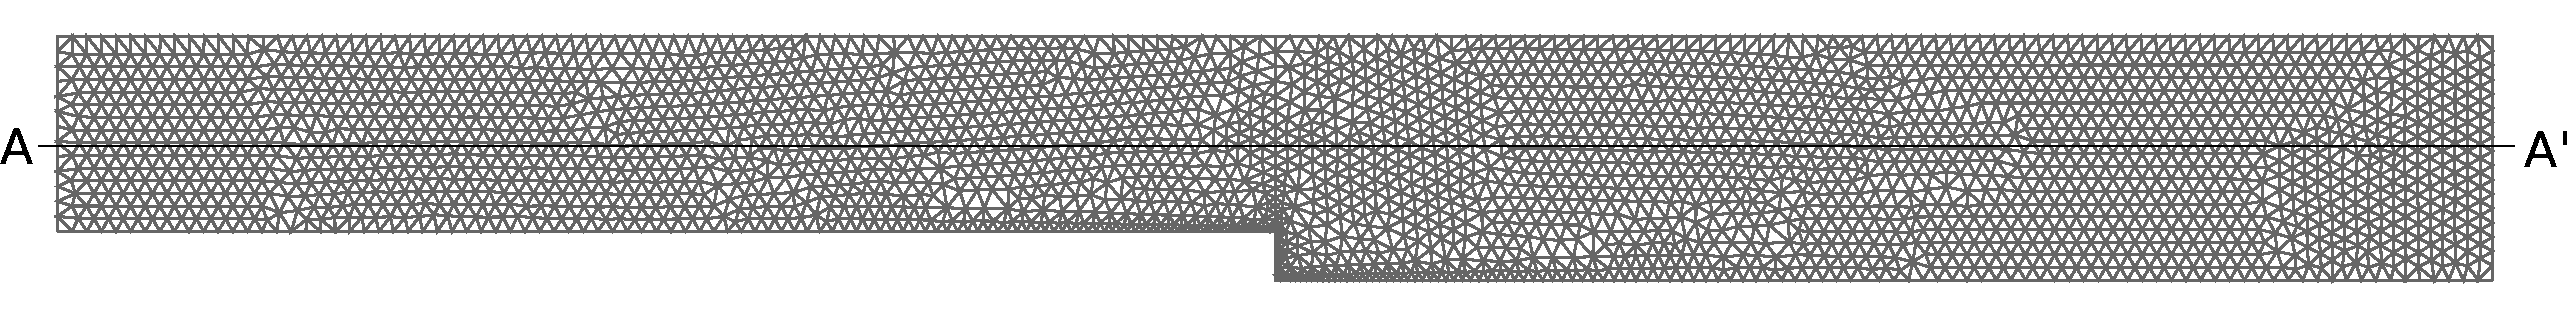
\includegraphics[width=\textwidth]{img/step/mesh.pdf}
    \caption{Definition of the domain and mesh used in the simulation. The average element size is $0.06m$, near the obstacle there is a mesh refinement to $0.02m$. There are $3.125$ nodes and $5.826$ elements.}
    \label{step_mesh}
\end{figure}

The problem is discretized with a mesh fine enough to test the artificial diffusion added by the stabilization. The average element size is $0.06m$ and near the corner the mesh is refined to $0.02m$.
The time step is set automatically to keep a Courant number equal to $1.0$ at every step. The problem is executed three times with different algorithmic constants $\beta = 0.001, 0.01, 0.1$. In that example, the shock capturing term is switch off.

\begin{figure}[H]
\begin{subfigure}{\textwidth}
    \centering
    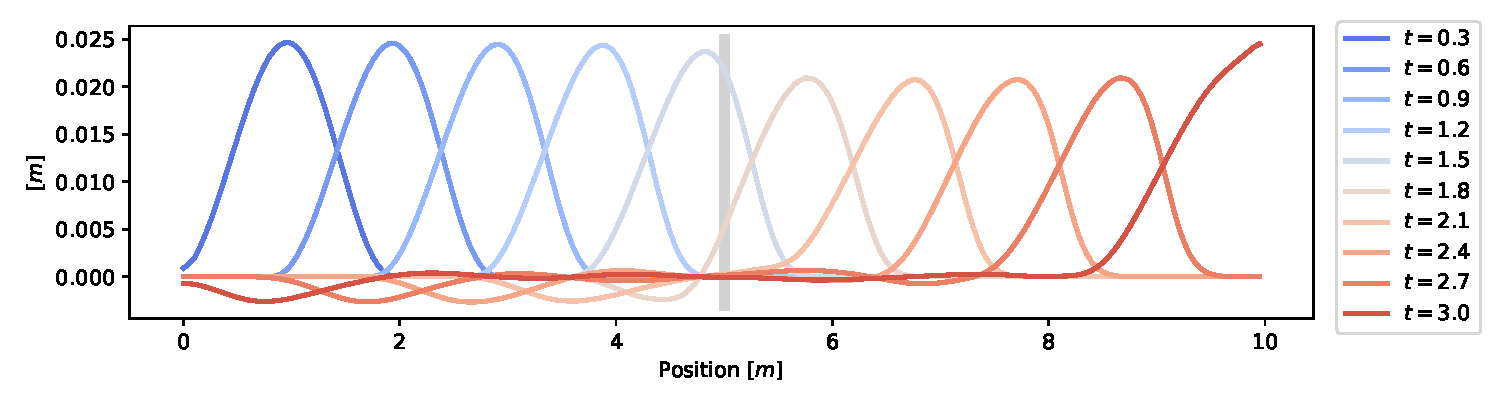
\includegraphics[width=\textwidth]{img/step/free_surface_1.pdf}
    \caption{Time from $0$ to $3s$}
\end{subfigure}
\begin{subfigure}{\textwidth}
    \centering
    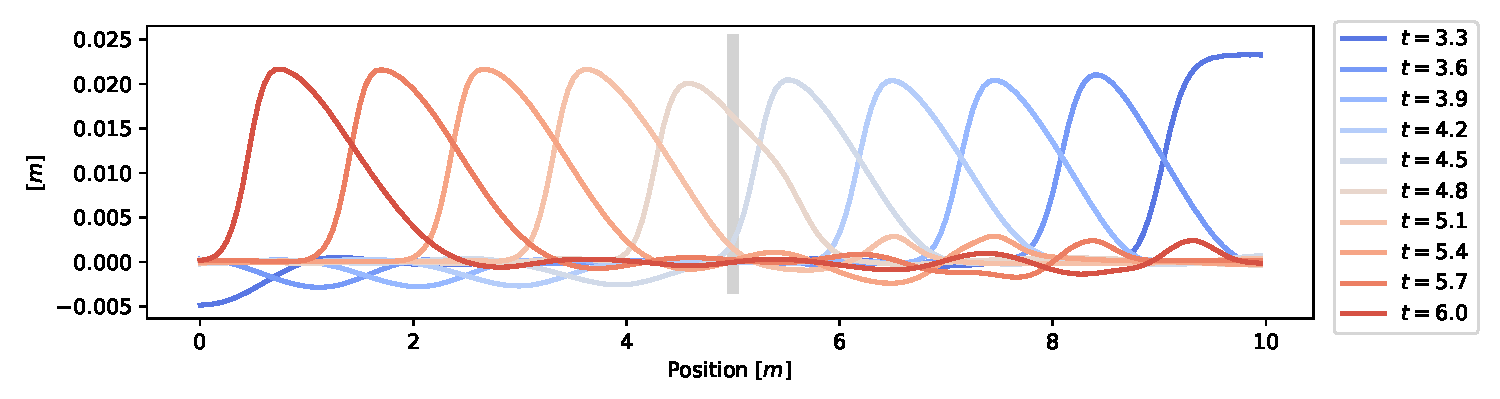
\includegraphics[width=\textwidth]{img/step/free_surface_2.pdf}
    \caption{Time from $3$ to $6s$}
\end{subfigure}
\caption{Timestamps of the free surface along the cut AA' from the figure(\ref{step_mesh}). In figure (a) the initial perturbation is propagating to the right. The results in figure (b) represent the propagation of the reflected wave from right to left.}
\label{waves_propagation}
\end{figure}


The best results are achieved with the intermediate value and it has been fixed for the rest of the examples in this paper.
In figures (\ref{stab_parameters_time1}) and (\ref{stab_parameters_time2}) can be observed that the lower value of $\beta$ is not enough to provide stability, while the higher value is over diffusive.


\begin{figure}[H]
\begin{subfigure}{.05\textwidth}
    \caption{}
\end{subfigure}
\begin{minipage}[c]{.94\textwidth}
    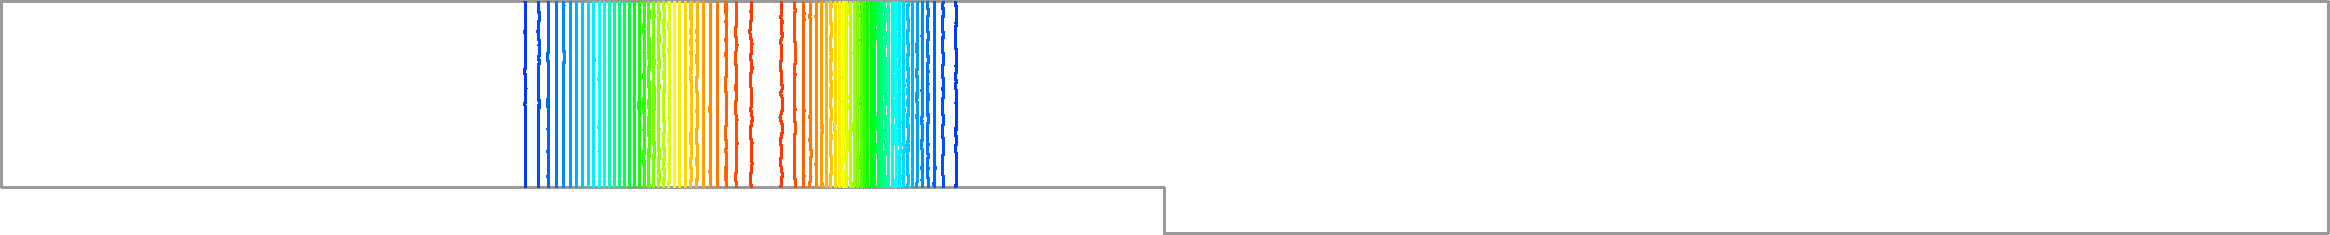
\includegraphics[width=\textwidth]{img/step/stab_0.001_time_1.pdf}        
\end{minipage}
\par\medskip
\begin{subfigure}{.05\textwidth}
    \caption{}
\end{subfigure}
\begin{minipage}[c]{.94\textwidth}
    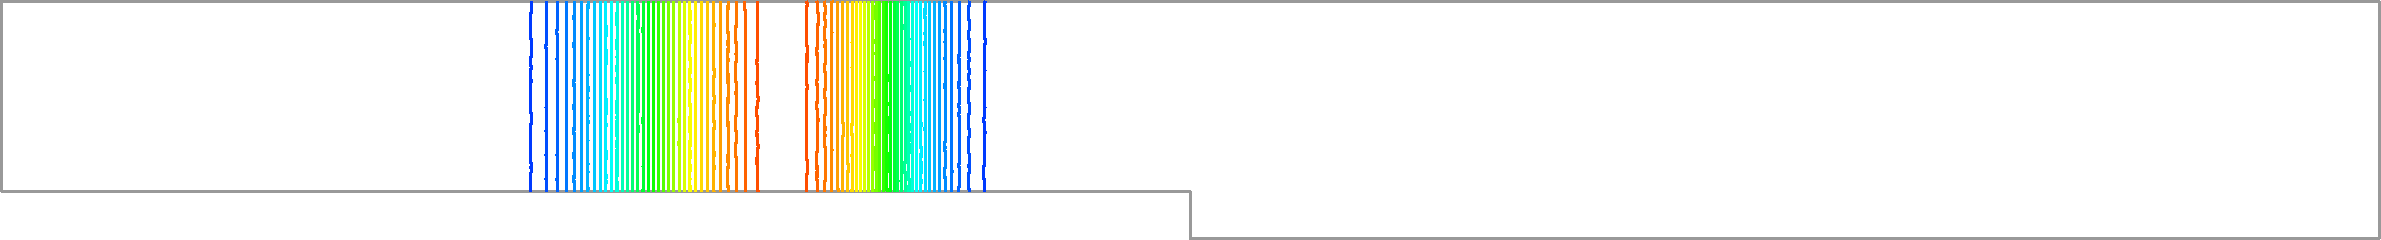
\includegraphics[width=\textwidth]{img/step/stab_0.01_time_1.pdf}        
\end{minipage}
\par\medskip
\begin{subfigure}{.05\textwidth}
    \caption{}
\end{subfigure}
\begin{minipage}[c]{.94\textwidth}
    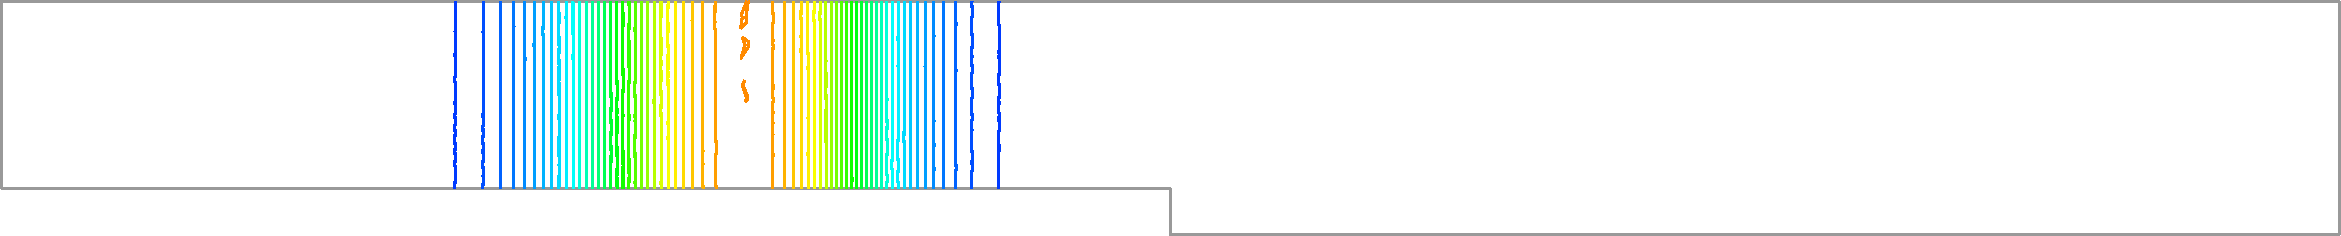
\includegraphics[width=\textwidth]{img/step/stab_0.1_time_1.pdf}        
\end{minipage}
\caption{Contour plots of the free surface elevation at time $t=1s$ for different stabilization factors. (a) $\beta=0.001$, (b) $\beta=0.01$, (c) $\beta=0.1$}
\label{stab_parameters_time1}
\end{figure}

\begin{figure}[H]
    \begin{subfigure}{.05\textwidth}
        \caption{}
    \end{subfigure}
    \begin{minipage}[c]{.94\textwidth}
        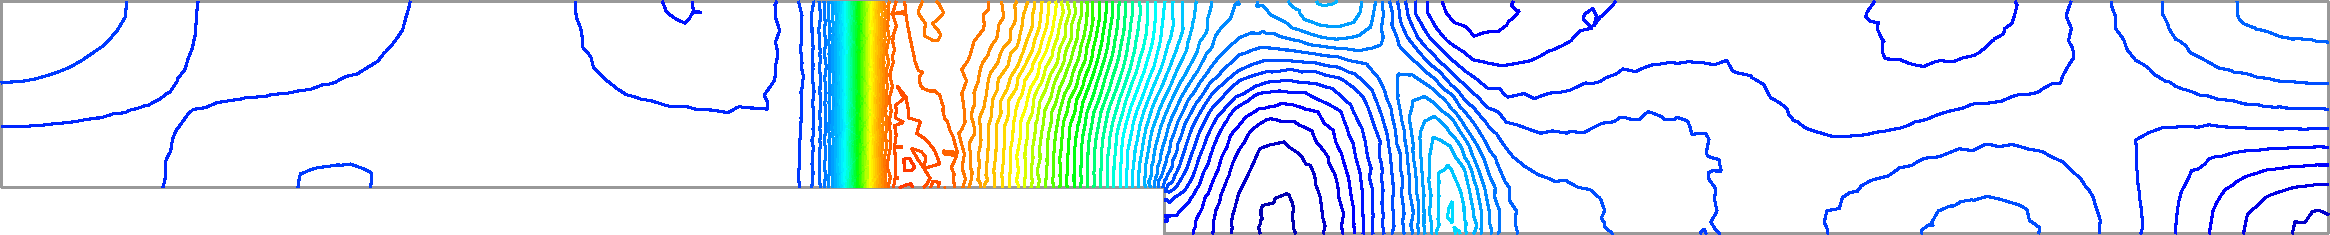
\includegraphics[width=\textwidth]{img/step/stab_0.001_time_5.pdf}        
    \end{minipage}
    \par\medskip
    \begin{subfigure}{.05\textwidth}
        \caption{}
    \end{subfigure}
    \begin{minipage}[c]{.94\textwidth}
        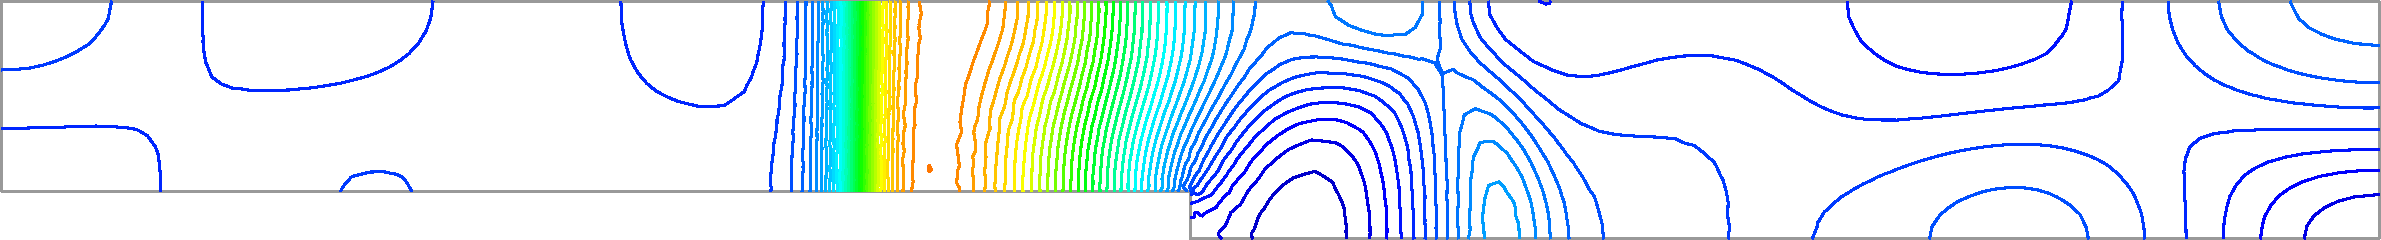
\includegraphics[width=\textwidth]{img/step/stab_0.01_time_5.pdf}        
    \end{minipage}
    \par\medskip
    \begin{subfigure}{.05\textwidth}
        \caption{}
    \end{subfigure}
    \begin{minipage}[c]{.94\textwidth}
        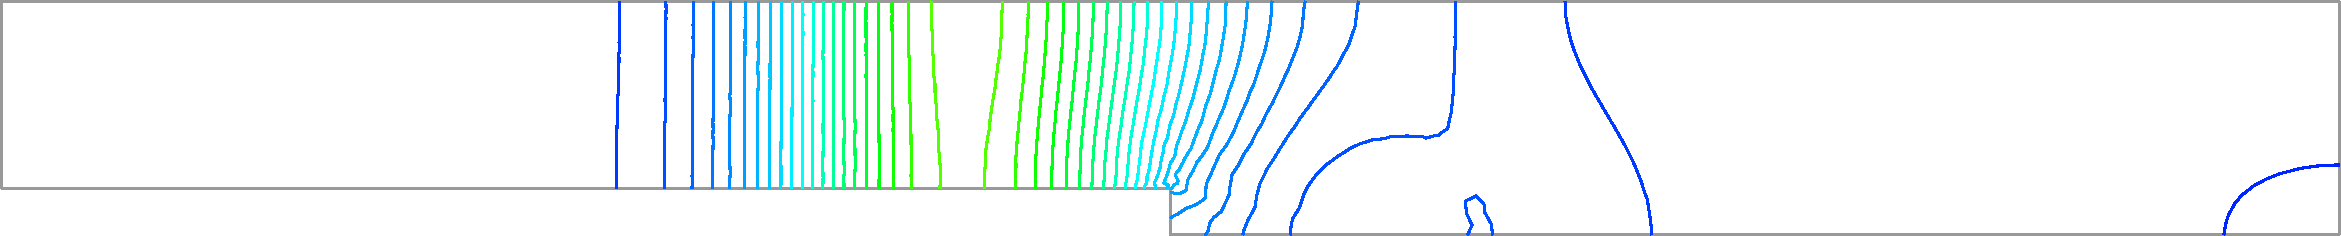
\includegraphics[width=\textwidth]{img/step/stab_0.1_time_5.pdf}        
    \end{minipage}
\caption{Contour plots of the free surface elevation at time $t=5s$ for different stabilization factors. (a) $\beta=0.001$, (b) $\beta=0.01$, (c) $\beta=0.1$}
\label{stab_parameters_time2}
\end{figure}



\subsection{Oscillation in a parabolic basin}

The second example is a classical benchmark oriented to test the accuracy of the location of the moving boundary. The topography follows a parabolic profile while the initial free surface elevation is planar and intersects the topography. The initial configuration corresponds to water at rest but the free surface is in a non horizontal plane. The solution of that problem is an oscillation where the free surface elevation remains planar. An analytical solution can be found in the compilation made by Delestre et al. \cite{delestre2013}.

The domain $\Omega$ is defined in the interval $[0,L]\times[0,1]m$ where $L=10$ and all the boundaries are reflective ($\mathbf{u}\cdot\mathbf{n} = 0$). The topography is given by the following expression
\begin{equation}
z(x,y) = h_0 \left(\frac{1}{a^2}\left(x - \frac{L}{2}\right)^2 - 1\right)
\end{equation}
and the primitive variables are defined by
\begin{subequations}
\begin{align}
h(x,y) &=
\begin{cases}
-h_0\left(\left(\frac{1}{a}\left(x - \frac{L}{2}\right) + \frac{1}{2a}\cos(2Bt)\right)^2 - 1\right)
\quad &\text{if} \ x_1(t) < x < x_2(t) \\
0 \quad &\text{otherwise}
\end{cases} \\
\mathbf{u}(x,y) &=
\begin{cases}
(B,0)\sin(2Bt) \quad &\text{if} \ x_1(t) < x < x_2(t) \\
(0,0) \quad &\text{otherwise}
\end{cases}
\end{align}
\end{subequations}
where $B=\sqrt{2gh_0}/2a$, and $x_1$, $x_2$ are time dependent functions which define the location of the dry-wet interface:
\begin{equation}
\begin{split}
x_1(t) = -\frac{1}{2}\cos(2Bt) - a + \frac{L}{2} \\
x_2(t) = -\frac{1}{2}\cos(2Bt) + a + \frac{L}{2}
\end{split}
\end{equation}

\begin{figure}
    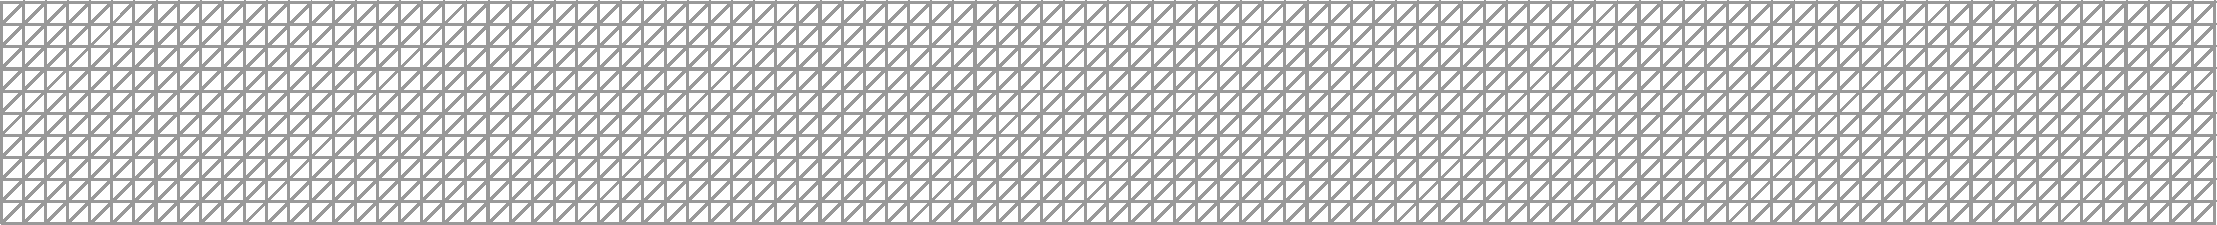
\includegraphics[width=\textwidth]{img/par/mesh_0.1.pdf}
    \caption{One of the meshes used to test the parabolic basin benchmark. The current element size is $0.1m$.}
    \label{parabola_mesh}
\end{figure}

\begin{figure}[H]
\begin{subfigure}{0.4\textwidth}
    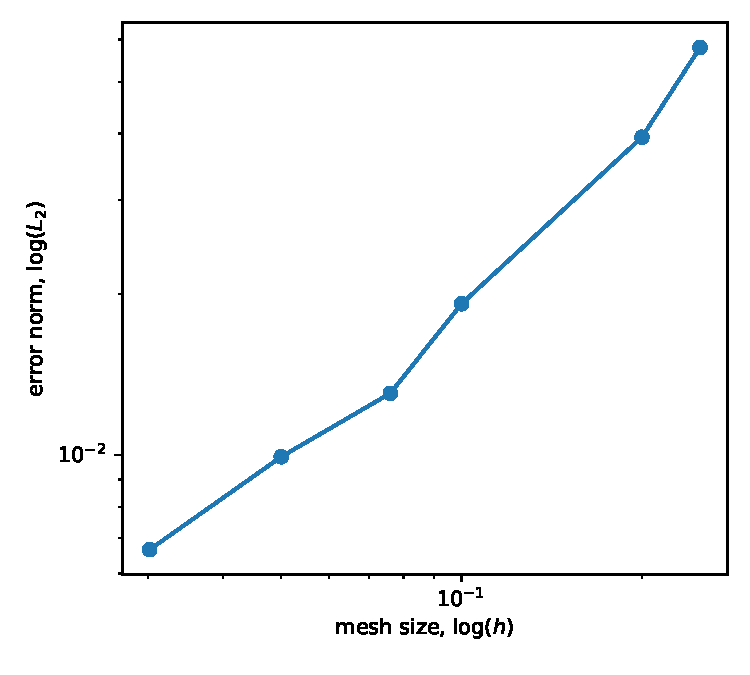
\includegraphics[width=\textwidth]{img/par/conv_1.pdf}    
\end{subfigure}
\hfill
\begin{subfigure}{0.58\textwidth}
    \begin{tabular}{+>{\small}r^c^c^c^c} \hline
    $n_{nodes}$ & $\Delta x$ & $\Delta t$ & CFL & $L_2(e_{rel})$ \\ \hline
205 & 0.25 & 0.008 & 0.5 & 0.24 \\
1,111 & 0.1 & 0.003 & 0.5 & 0.064 \\
4,221 & 0.05 & 0.002 & 0.5 & 0.023 \\
11,356 & 0.03 & 0.001 & 0.5 & 0.013 \\
101,101 & 0.01 & 0.0003 & 0.5 & 0.0049 \\
    \hline
    \end{tabular}
\end{subfigure}
\caption{Convergence analysis for the parabolic basin benchmark}
\label{parabola_convergence}
\end{figure}

\begin{figure}[H]
\begin{subfigure}{\textwidth}
    \centering
    Time $t=0.5s$
    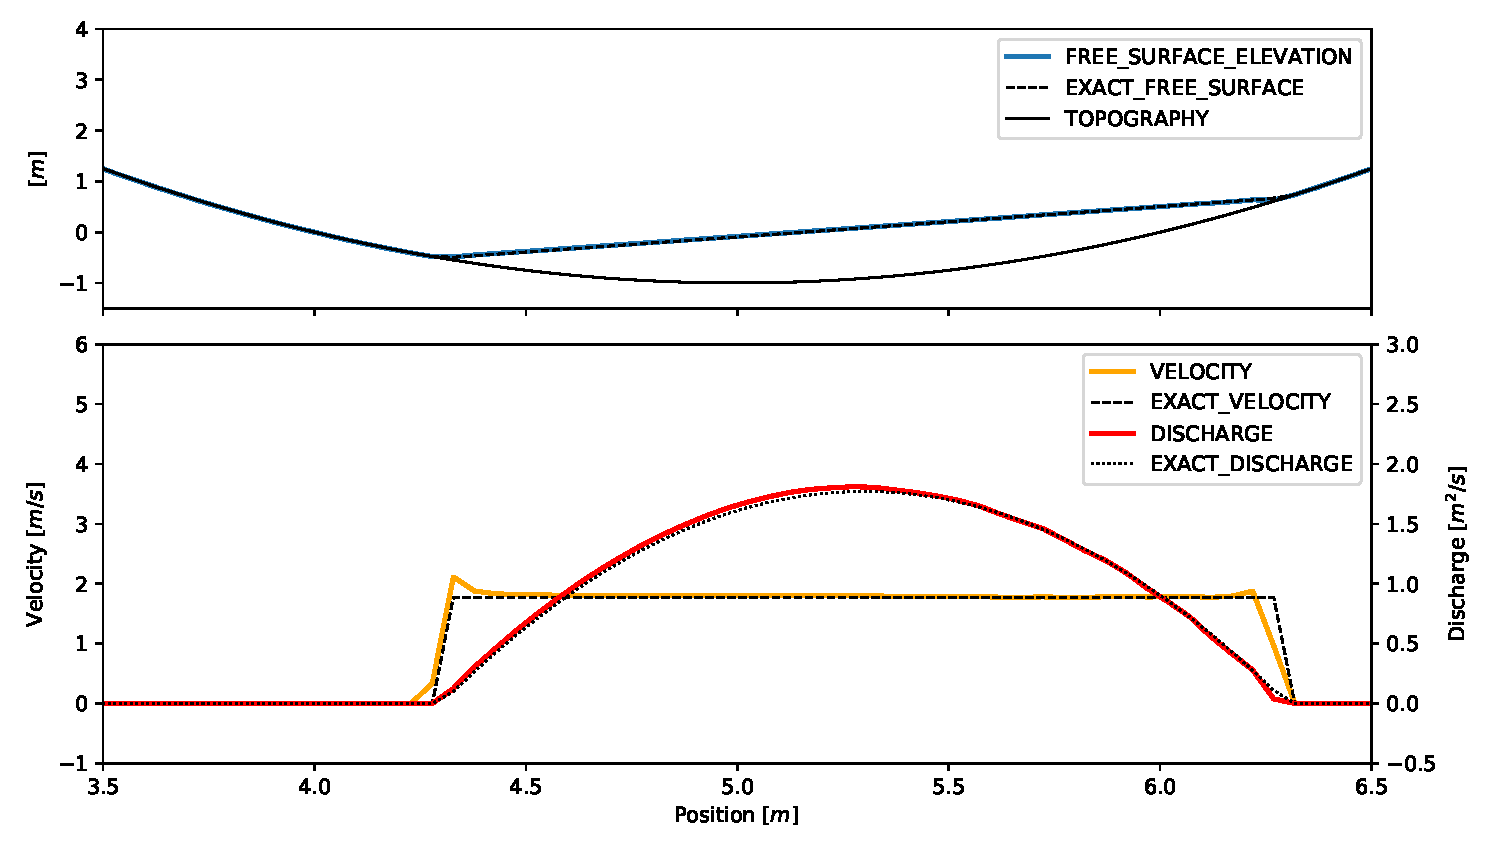
\includegraphics[width=\textwidth]{img/par/parabola_t0.5.pdf}
\end{subfigure}
\par\medskip
\begin{subfigure}{\textwidth}
    \centering
    Time $t=1s$
    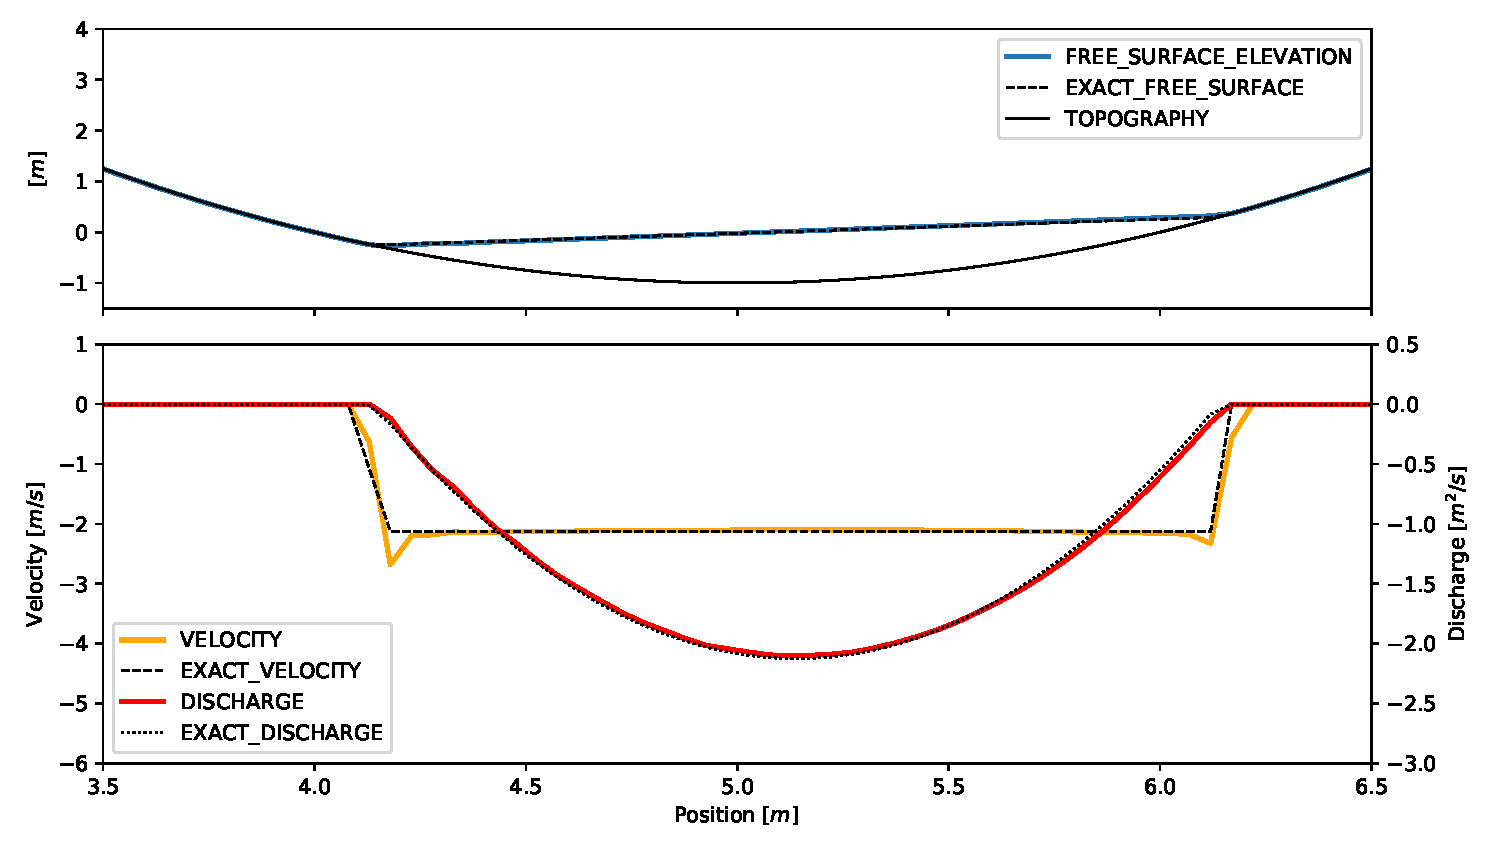
\includegraphics[width=\textwidth]{img/par/parabola_t1.0.pdf}
\end{subfigure}
\caption{Cuts along the mesh of size $0.03m$ at different times. There are 333 nodes on the cut.}
\label{parabola_graphic}
\end{figure}

\begin{figure}[H]
\begin{subfigure}{\textwidth}
    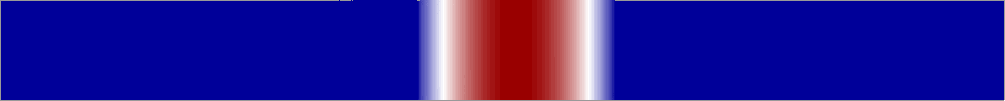
\includegraphics[width=\textwidth]{img/par/height_1.0.png}
\end{subfigure}
\par\medskip
\begin{subfigure}{\textwidth}
    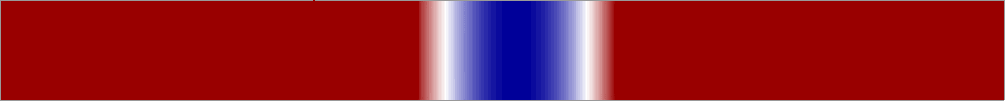
\includegraphics[width=\textwidth]{img/par/momentum_1.0.png}
\end{subfigure}
\par\medskip
\begin{subfigure}{\textwidth}
    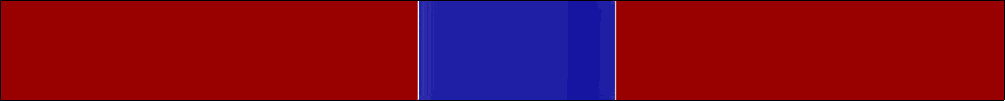
\includegraphics[width=\textwidth]{img/par/velocity_1.0.png}
\end{subfigure}
\caption{Results with the fie mesh of size $0.01m$ at time $t=1s$. The images display the water height at the top, the x-discharge at the middle and the x-velocity below. There is not legend for simplicity, the red colour is positive and blue means a null or negative magnitude.}
\label{parabola_results}
\end{figure}



\subsection{Short channel with smooth transition and shock}

The third example in a benchmark based on the Mac Donald's type solutions \cite{macdonald1997}. The analytical solution also can be found in the same compilation than the previous example \cite{delestre2013}. This test presents channel with a steady state solution. There is a subcritical inlet in a region where a transcritical flow is produced. The outlet is also subcritical and a shock is generated at $\sfrac{2}{3}$ of the channel. The aim of this example is to evaluate the presented shock capturing technique and the correct location of the hydraulic jump.

Here we will consider the one-dimensional shallow water equations without diffusion and only with Manning bottom friction as source term. A steady state solution satisfies $\pder{q}{x}=0$ and the equation (\ref{general_sw}) reduces to
\begin{equation} \label{steady_state}
\pder{z}{x} = \left(\frac{v^2}{gh}-1\right) \pder{h}{x} - n^2\frac{\abs{v}v}{h^{\sfrac{4}{3}}}
\end{equation}
This relation allows to integrate the topography given an analytical expression for the water height. Another approach in hydraulics is to consider a given discharge and topography and integrate the water height using the relation (\ref{steady_state}). In both approaches exact solutions can be obtained. Since this expression involves the bottom friction, we can prove if the friction term is coded in order to satisfy the steady state.

For this benchmark we have considered the domain defined by the interval $[0,100]\times[0,5]$ which is a channel of $100m$ length and $5m$ width, and the following boundary conditions:
\begin{equation}
\begin{split}
    q_x = 2\ \text{m/s} \qquad &\text{in} \ \Gamma_{upstream} \\
    h = h_{ex}(100) \qquad &\text{in} \ \Gamma_{downstream} \\
    q_y = 0 \qquad &\text{in} \ \Gamma_{walls}
\end{split}
\end{equation}
The Manning coefficient is $0.0328\ \text{m}^{-1/3}\text{s}$ and the water height $h_{ex}(x)$ is a piecewise function defined in \cite{delestre2013}. The discontinuity of the water height function is located at $x=200/3\ m$ and defines the hydraulic jump.

\begin{figure}
    
\includegraphics[width=\textwidth]{img/jump/sketch/sketch.pdf}
    \caption{Geometry of the channel, the vertical line shows the position of the hydraulic jump, the shadowed area correspond to the location where the $L_2$ norm of the error is computed.}
\end{figure}


\begin{figure}[H]
\begin{subfigure}{0.4\textwidth}
    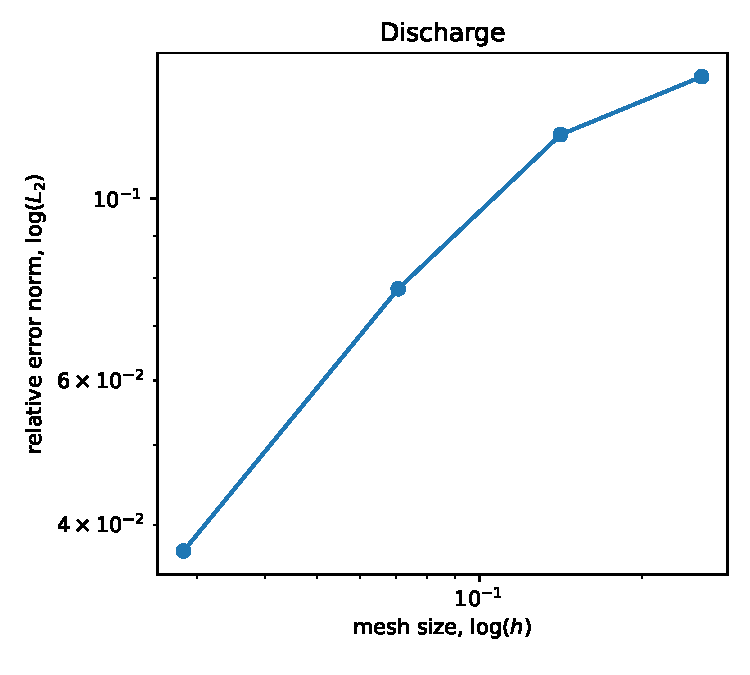
\includegraphics[width=\textwidth]{img/jump/momentum_convergence.pdf}    
\end{subfigure}
\hfill
\begin{subfigure}{0.58\textwidth}
    \begin{tabular}{+>{\small}r^c^c^c^c} \hline
    $n_{nodes}$ & $\Delta x$ & $\Delta t$ & CFL   & $L_2(e_{rel})$ \\ \hline
    204         &        2.0 &      0.005 & 0.016 & 0.177 \\
    606         &        1.0 &      0.005 & 0.031 & 0.138 \\
    2211        &        0.5 &      0.005 & 0.062 & 0.088 \\
    13026       &        0.2 &      0.005 & 0.15  & 0.041 \\ \hline
    \end{tabular}
\end{subfigure}
\caption{Convergence analysis for the short channel with smooth transition and shock.}
\label{hydraulic_jump_convergence}
\end{figure}


\begin{figure}
    \centering
    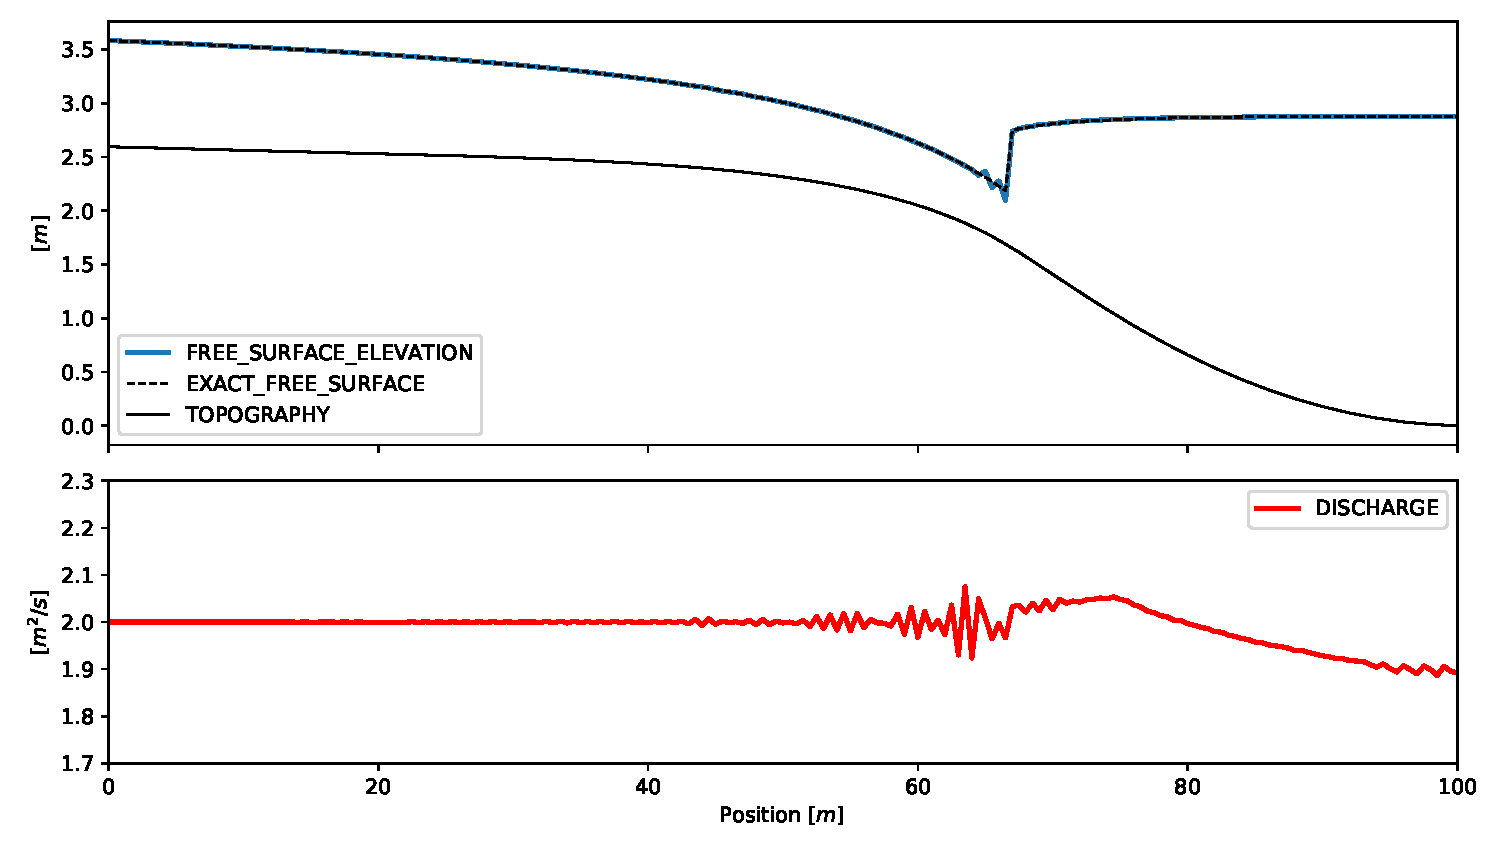
\includegraphics[width=\textwidth]{img/jump/mesh_0.5.pdf}
    \caption{Graph along the cut defined by the center of the channel. The mesh size is $0.5m$}
    \label{mac_donald_shock_graph_5}
\end{figure}

\begin{figure}
    \centering
    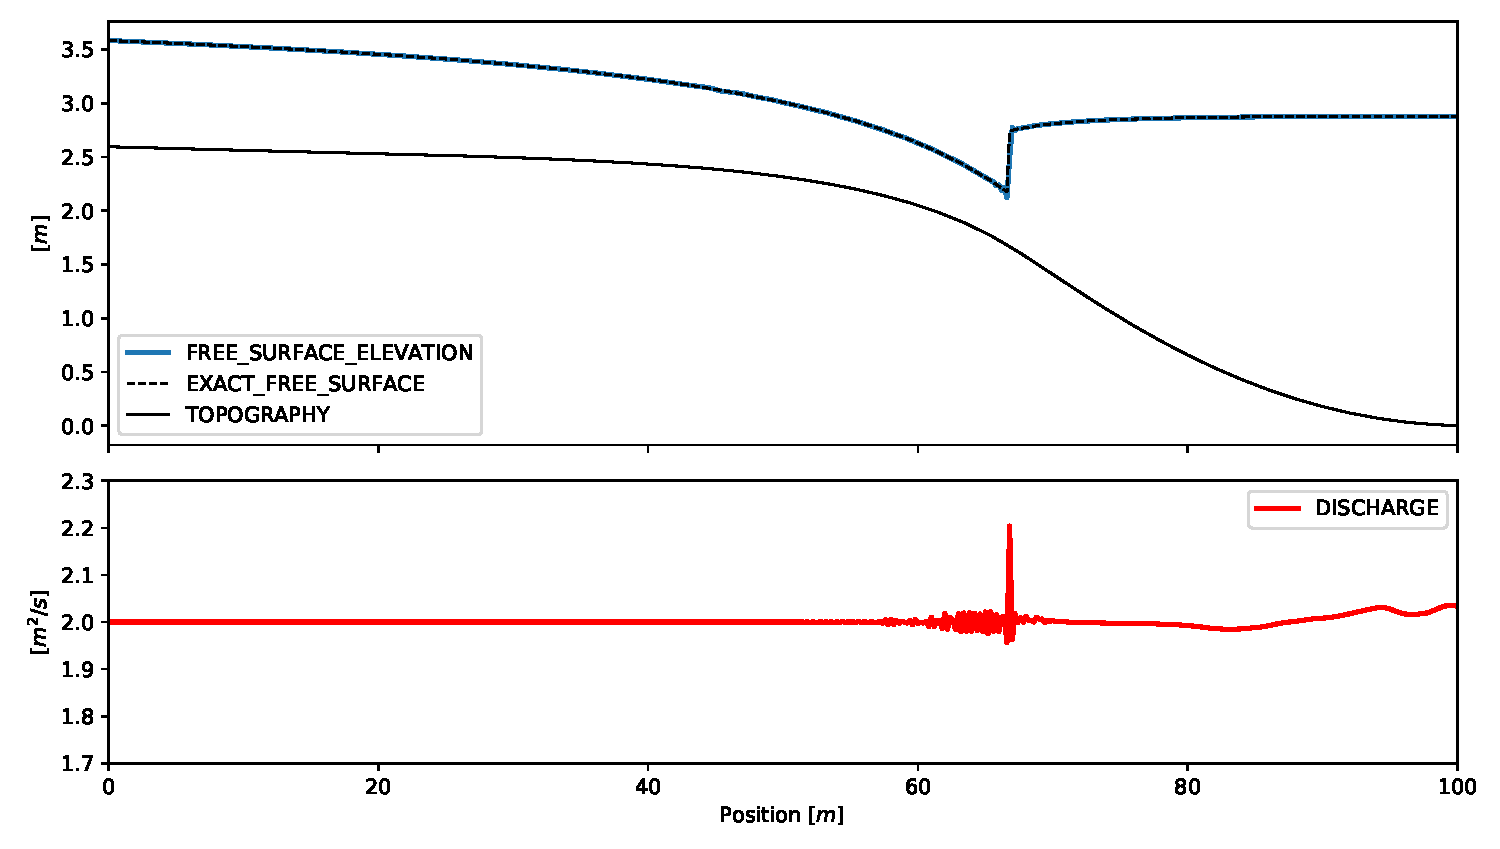
\includegraphics[width=\textwidth]{img/jump/mesh_0.2.pdf}
    \caption{Graph along the cut defined by the center of the channel. The mesh size is $0.2m$}
    \label{mac_donald_shock_graph_2}
\end{figure}


\subsection{Experimental dam break flow against an isolated building}

The last example consists on the reproduction of the experiment carried out by Soares \cite{soares2007}.
A dam break flow with a building downstream is simulated and the problem definition is depicted in figure \ref{experiment_sketch}. The channel is $3.4m$ width and the end of the dam is located at $x=0$.
As initial conditions, the water depth is set to $0.4m$ in the reservoir, the channel is dry. The manning coefficient is $0.01ms^{-1}$ over all the domain.
At the beginning of the simulation, the gate of the dam is removed and the water is allowed to flow around the building.

Figure \ref{experiment_plots} shows several results of the water depth after the gate release and figure \ref{experiment_gauges} shows the evolution of the water depth at the gauges. An initial delay is observed in the propagation of the front in the gauges 1 to 5.
The gauges 1 and 2 show a rise of the water level after the first front is arrived, this behavior correspond to the hydraulic jump generated in front of the building.
Regarding the performance of that formulation, it captures the main aspects of the flow, but not the details, since there are some regions on that experiment which violate the shallow water approximations.

\begin{figure}[H]
\centering
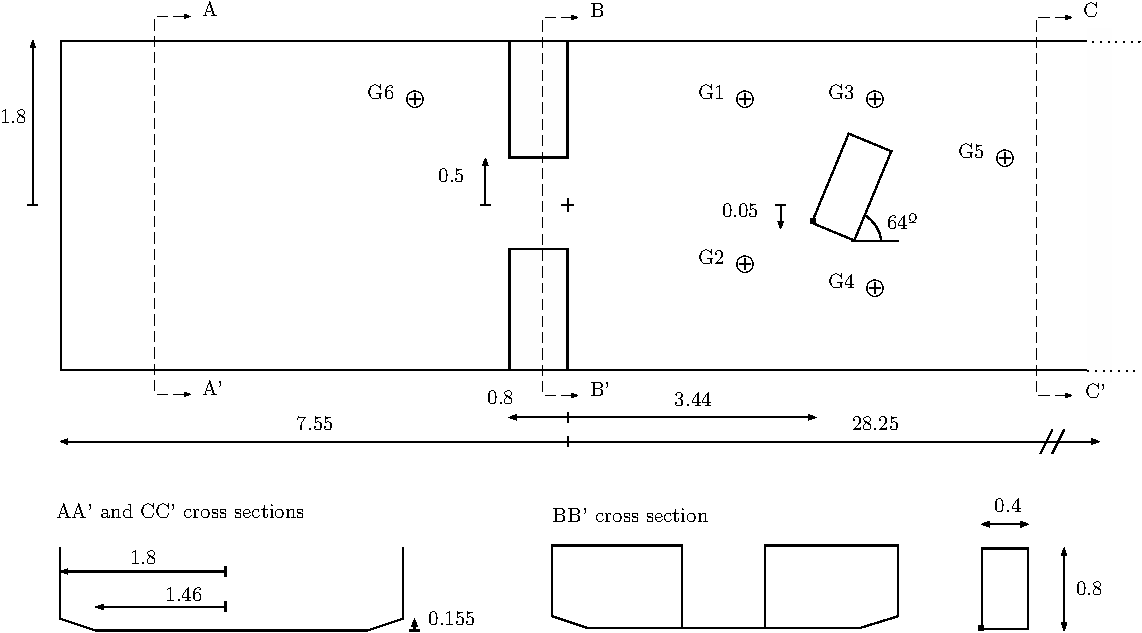
\includegraphics[width=\textwidth]{img/exp/sketch.pdf}
\caption{Definition of the isolated building benchmark. The dimensions are in $m$.}
\label{experiment_sketch}
\end{figure}


\begin{figure}[H]
\centering
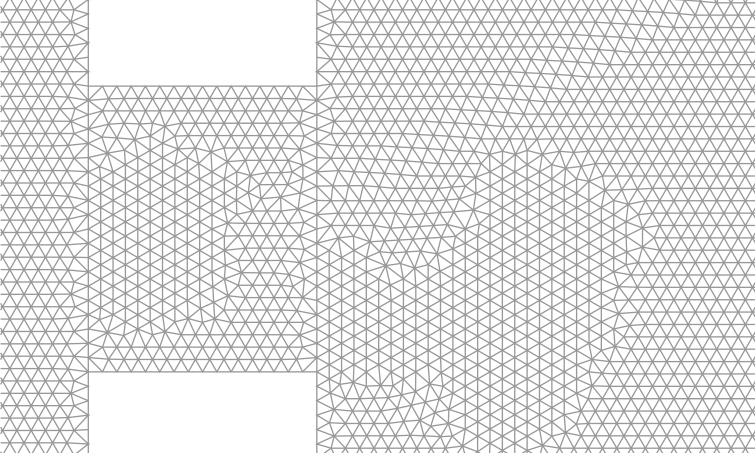
\includegraphics[width=.49\textwidth]{img/exp/mesh_dam.png}
\hfill
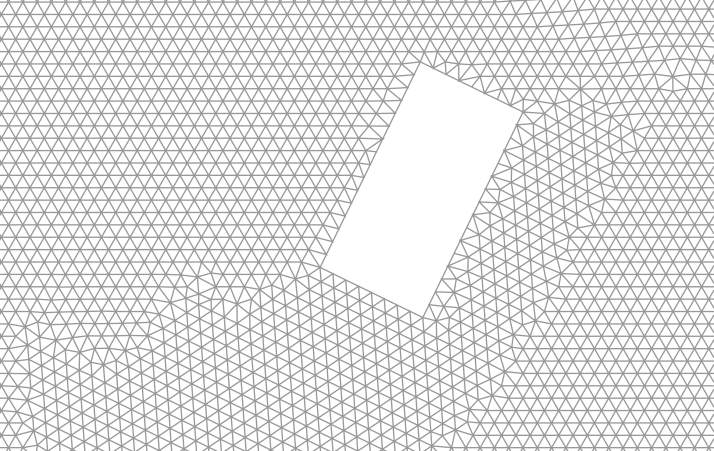
\includegraphics[width=.47\textwidth]{img/exp/mesh_building.png}
\caption{Details of the mesh around the dam and around the building. The average mesh size is $0.05m$ and there are 115.000 elements.}
\label{experiment_mesh}
\end{figure}


\begin{table}
\centering
\begin{tabular}{ccc}
\hline
Gauge number & X & Y \\ \hline
1 &  2.65 &  1.15 \\
2 &  2.65 & -0.60 \\
3 &  4.00 &  1.15 \\
4 &  4.00 & -0.80 \\
5 &  5.20 &  0.30 \\
6 & -1.87 &  1.10 \\ \hline
\end{tabular}
\caption{Positions of the gauges, units in $m$.}
\label{gauges_positions}
\end{table}


\begin{figure}
\centering
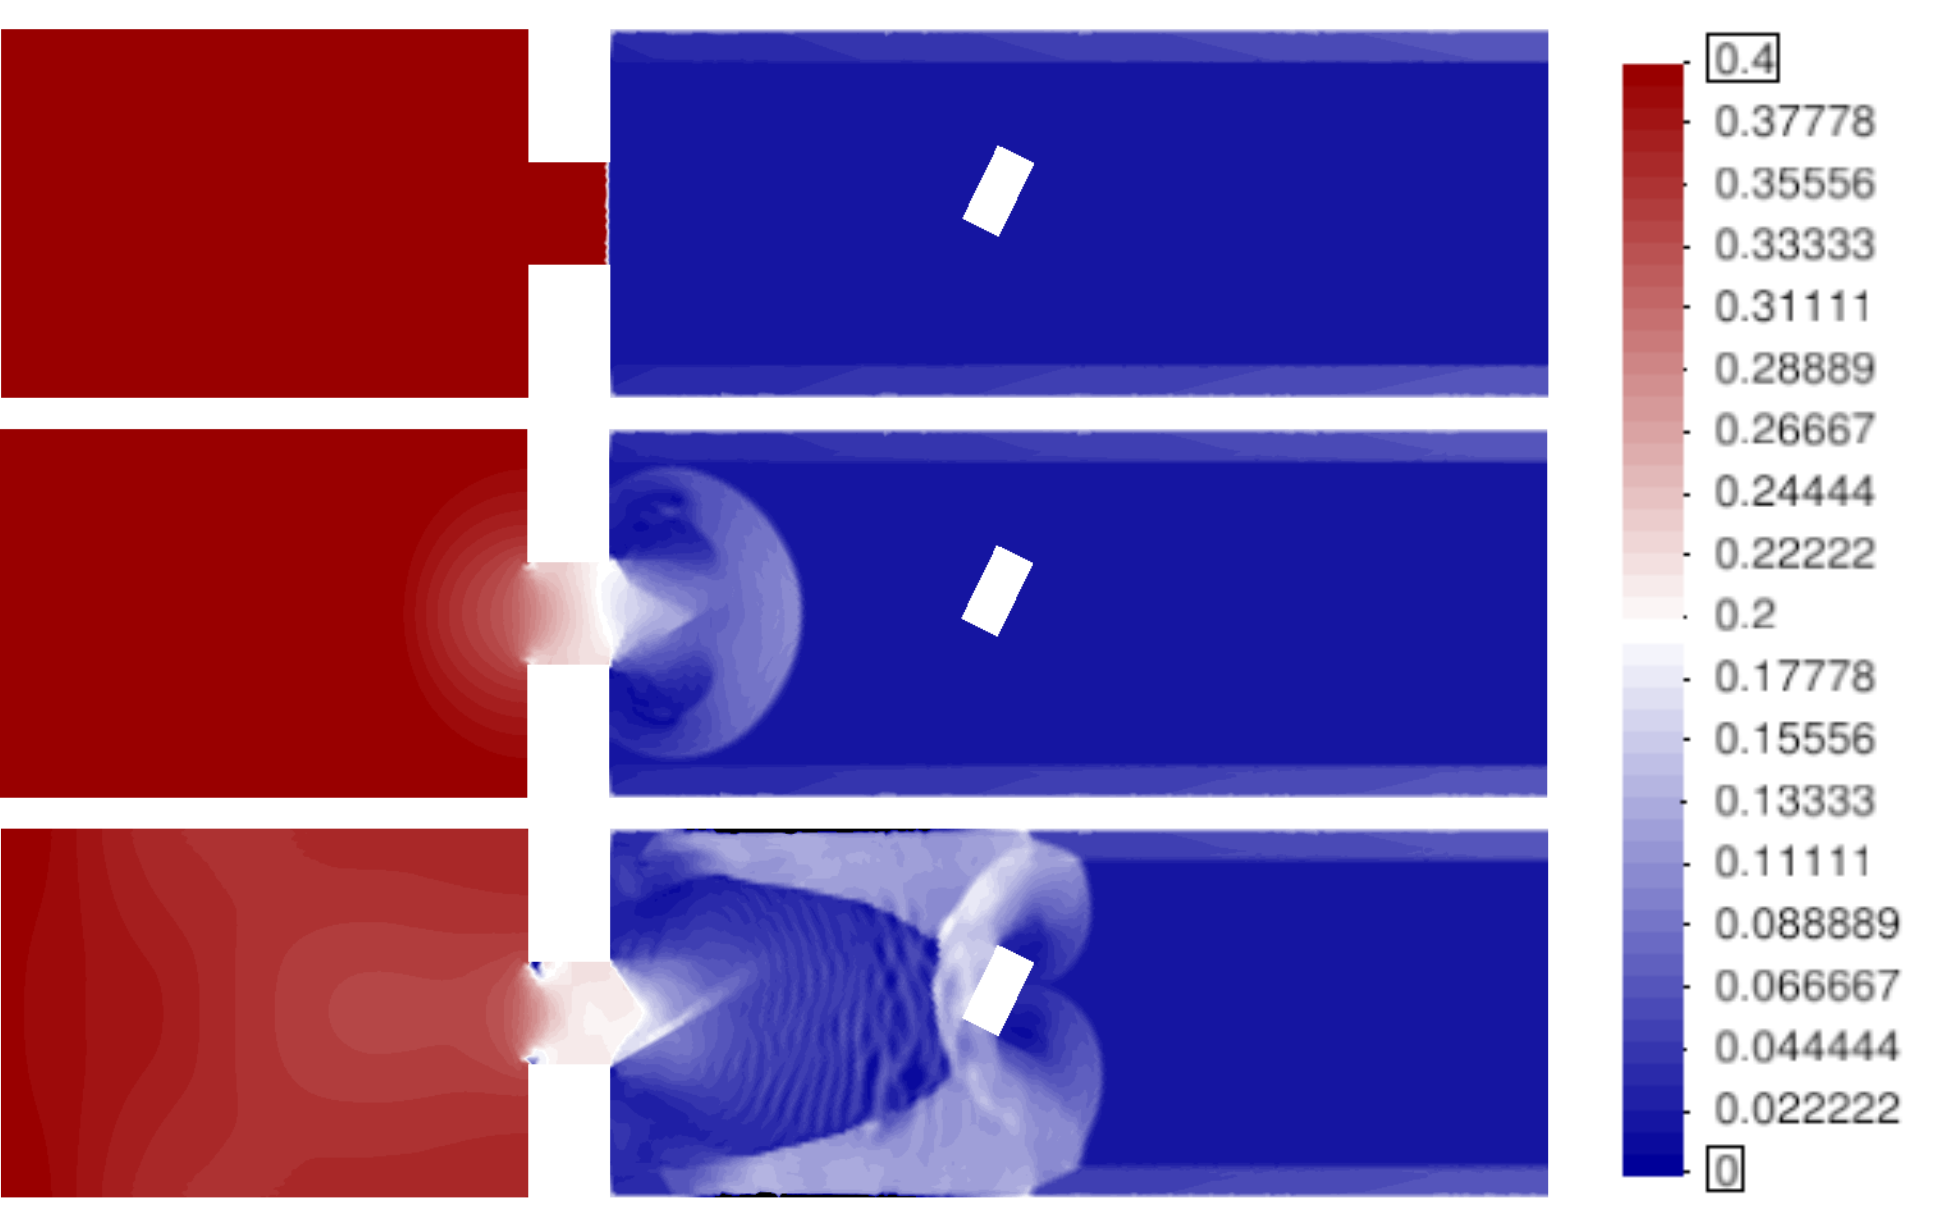
\includegraphics[width=\textwidth]{img/exp/results.png}
\caption{Results of the benchmark at times $0$, $1$ and $3$ seconds}
\label{experiment_plots}
\end{figure}


\begin{figure}
\centering
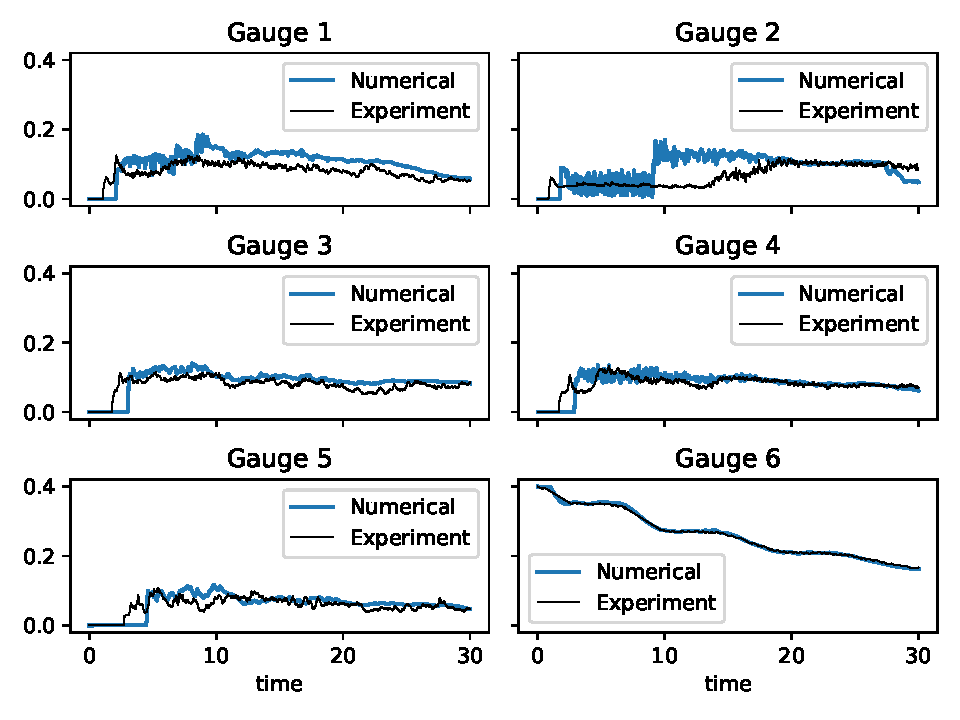
\includegraphics[width=\textwidth]{img/exp/gauges.pdf}
\caption{Comparison between the obtained water depth with the reference data.}
\label{experiment_gauges}
\end{figure}



\section{Concluding remarks} \label{sec:conclusions}

We have extended the FIC-FEM procedure to the shallow water equations. Unlike the FIC-based stabilizations for incompressible flows, the present procedure is applied to the coupled mass and momentum balance at the same time using the linearization matrix $\mathbf{A}_i$. It can be seen that this procedure casts to the classical FIC-stabilization for convection diffusion problems, taking the velocity $u_i$ as linearization term. The same procedure can be applied to develop stabilized formulations for compressible flows.
%Compared to the FIC-based stabilized formulations for incompressible flows, the FIC-FEM procedure should be applied to the coupled mass and momentum balance. The same procedure can be applied to develop stabilized formulations for compressible flows.\Miguel{NO SE SI S'ENTÉN AIXÒ: QUE NO ES POT ESTABILITZAR EL MOMENT PER UNA BANDA I LA MASSA PER L'ALTRA BANDA} \Ignasi{ESTIC D'ACORD, FES UNA ACLARACIO D'AIXO}

((Even though this method presents an equivalent structure as SUPG, a more general framework can be explored with the VMS formulation, which includes the linearization matrices of the viscous terms and reaction terms. However, since the shallow water equations are dominated by the convective matrix $\mathbf{A}_i$, and thus are strictly hyperbolic, the present stabilization is enough to provide stability.)) \Ignasi{NO ENTENC PERQUE PARLES DE L'ESTABILITZACIO VMS AQUI. HA DE QUEDAR CLAR QUINA ES L'APORTACIO DEL PAPER EN RELACIO A L'ESTABILITZACIO PRESENTADA} \Miguel{AQUÍ ESTIC PARLANT DEL LIMITS DE L'APORTACIÓ.}

The present stabilization provides two algorithmic constants, one for the global stabilization and other one for the shock capturing term. From our numerical experiments, we have chosen $\beta=0.01$ for the stabilization and $\alpha=1.0$ for the shock capturing. \IgnasiCorregit{REVISA QUE NO HAGIS REPETIT EL SIMBOL $\alpha$ PER A VARIS SIGNIFICATS}

The present FIC-FEM procedure has been able to produce accurate results for the examples considered.
In the first example, the artificial diffusion is evaluated and it has been proved to be small and practically inappreciable. The shock capturing allows to solve supercritial problems with discontinuities and the present procedure is also able to deal with partially wet domains. Finally, a numerical simulation of a dam break flow against an isolated building is performed showing a good agreement with the experimental data.
\IgnasiCorregit{JO AFEGIRIA UN PETIT PARAGRAF RESUMINT ELS RESULTATS OBTINGUTS ALS EXEMPLES. (NO DETALLAT, NOMES UNES PINCELLADES)}



\section{Acknowledgements}

This research was partially funded by the projects (...). The authors also acknowledge the financial support from the CERCA programme of the Generalitat de Catalunya, Spain, and from the Spanish Ministry of Economy and Competitiveness, through the “Severo Ochoa Programme for Centres of Excellence in R\&D”, Spain (CEX2018-000797-S).



\section*{Appendix A}
\addcontentsline{toc}{section}{Appendix A}

The stabilization matrices ere the result of multiplying $\mathbf{A}$ tensor by itself:

\begin{subequations}
\begin{equation}
\mathbf{A}_1\mathbf{A}_1 =
\begin{pmatrix}
3u_1^2 + c^2 & 0  & -2u_1^3 + 2u_1c^2 \\
2u_1u_2  & u_1^2  & -2u_1^2u_2 + u_2c^2 \\
2u_1  & 0   & -u_1^2 + c^2
\end{pmatrix}
\end{equation}
\begin{equation}
    \mathbf{A}_2\mathbf{A}_2 =
\begin{pmatrix}
u_2^2  & 2u_1u_2  & -2u_1u_2^2 + u_1c^2 \\
0    & 3u_2^2 + c^2 & -2u_2^3 + 2u_2c^2 \\
0  & 2u_2  & -u_2^2 + c^2
\end{pmatrix}
\end{equation}
\begin{equation}
\mathbf{A}_1\mathbf{A}_2 =
\begin{pmatrix}
2u_1u_2  & u_1^2 + c^2  & -2u_1^2u_2 \\
u_2^2  & 2u_1u_2  & -2u_1u_2^2 + u_1c^2 \\
u_2  & u_1  & -u_1u_2
\end{pmatrix}
\end{equation}
\begin{equation}
\mathbf{A}_2\mathbf{A}_1 =
\begin{pmatrix}
2u_1u_2  & u_1^2  & -2u_1^2u_2 + u_2c^2 \\
u_2^2 + c^2  & 2u_1u_2  & -2u_1u_2^2 \\
u_2  & u_1  & -u_1u_2
\end{pmatrix}
\end{equation}
\end{subequations}


\bibliography{../bibliography/sw}
\bibliographystyle{ieeetr}

\end{document}
